\documentclass[a4paper,man,floatsintext,natbib,donotrepeattitle, apacite]{apa6}
\usepackage{authblk}
\usepackage[utf8]{inputenc}
\usepackage{rotating} % provides sidewaystable and sidewaysfigure
\usepackage{natbib}
\bibliographystyle{apa}
\usepackage{bibentry}
\setcitestyle{notesep={; },round,aysep={},yysep={;}}
\usepackage[T1]{tipa}
\usepackage{amsmath}
\usepackage{enumitem}
\usepackage{makecell}
\usepackage{array}
\usepackage{float}
\usepackage{rotating}
\geometry{reset, letterpaper, height=9in, width=7in, hmarginratio=1:1, vmarginratio=1:1, marginparsep=0pt, marginparwidth=0pt, headheight=15pt}
\newcolumntype{P}[1]{>{\centering\arraybackslash}c{#1}}
\usepackage{bm}
\usepackage{tikz}
\usepackage{lmodern}
\usepackage{lipsum,ragged2e}% justify paragraphs
\usepackage{setspace}
\usepackage{endnotes} % put footnotes at end of paper
\usepackage{hyperref}

\let\footnote\endnote
\title{\LARGE Word structure in early Quechua speech: \\ Coarticulation and inflectional morphology}
\shorttitle{Early Quechua Speech}

\usetikzlibrary{shapes.geometric, arrows,backgrounds,fit,positioning}

\author[a]{\large Margaret Cychosz}

\affil[a]{\small University of California, Berkeley, Department of Linguistics, 1203 Dwinelle Hall, Berkeley, USA, \url{mcychosz@berkeley.edu}}
\affiliation{} % to remove weird affiliation

\abstract{Evidence from acoustic and articulatory phonetics increasingly suggests that morphological structure is reflected in spoken language patterns. For child language, this interaction between word structure and speech production has the potential to shed considerable light on the status of children’s early word forms - but the topic remains underexplored in child speech. How do children analyze the internal structure of morphologically complex words throughout childhood? To answer this, the current study measured the coarticulation patterns of bilingual Quechua-Spanish children (5-10 years) and adults. Coarticulation was measured acoustically in two word environments, within morphemes and across morpheme boundaries. Both child and adult participants distinguished coarticulatorily between the word environments, but they did so in different ways. Children differentiated between environments via a combination of duration and coarticulation while adults consistently coarticulated more in shorter duration sequences. Additionally, the children’s speech patterns, but not the adults’, were sensitive to prosodic structure: children produced increasingly shorter phones in words with more syllables. It was suggested that the difference between adults and children could be attributable to adults' faster speaking rate and increased dominance in Quechua.  Future work is needed to determine if young children's speech patterns reflect prosodic planning, morphological planning, or both.}

\keywords{coarticulation; morphophonetics; field phonetics; first language acquisition; morphology; Quechua}


\clearpage

\begin{document}
\justifying
\setlength\parindent{24pt} % indent each paragraph

\maketitle

\setcounter{secnumdepth}{2} % number sections


\section{Introduction}

Adult speakers can readily compose novel, morphologically complex word forms like \textit{daxy} or \textit{unraxlike} from morphemic subcomponents. Since \citet{berkoChildLearningEnglish1958} introduced the Wug Test, developmental researchers have acknowledged that young children must share this productive ability; if not, children would not be able to extend morphophonological patterns to novel lexical environments. Yet disagreement concerning children’s early linguistic representations, and thus how children form morphologically complex words, remains. Children's lexical forms could be fully adult-like from early toddlerhood (e.g. \citealt{wexlerVeryEarlyParameter1998}), the forms could emerge over time with usage (e.g. \citealt{ambridgeUbiquityFrequencyEffects2015}), or there could be some combination of the two approaches (e.g. \citealt{swingleyLexicalNeighborhoodsWordForm2002}). 

One window into the nature of lexical access and storage - at least in adult speakers - is to examine the effects of morphological structure on speech production. The complex relationship between speech variability and morphological structure in children is still relatively underexplored (cf. \citealt{redfordGrammaticalWordProduction2018}; \citealt{songEffectsCoarticulationMorphological2013}; \citealt{songDurationalCuesFricative2013}). Yet measuring how morphological structure is reflected in children's speech could allow us to infer about the status of children's early complex word forms. Are words that, to an adult are transparently morphologically complex, treated as such by children? And when a child does recognize that a given word is morphologically complex, how does this recognition affect children's lexical storage, access, and production? 

This study takes advantage of known relationships between acoustics, specifically coarticulation and phone duration, and word structure. The goal is to evaluate how the composition of morphologically complex words is reflected in speech production patterns in Quechua, a highly agglutinating language with over 200 productive verbal and nominal suffixes. In doing so, this work follows a growing line of research evaluating relationships between morphology and speech production (e.g. \citealt{choEffectsMorphemeBoundaries2001};  \citealt{hayCausesConsequencesWord2003}; \citealt{lee-kimMorphologicalEffectsDarkness2013}; 
\citealt{plagPhonologicalPhoneticVariability2014};  \citealt{songDurationalCuesFricative2013}; \citealt{songEffectsCoarticulationMorphological2013}; 
\citealt{strycharczukPhoneticDetailPhonetic2019};
\citealt{tomaschekHowAnticipatoryCoarticulation2019}). Here, coarticulation is measured across and within morpheme boundaries in adults and a cross-sectional cohort of school-aged children to examine if, and how, speakers distinguish coarticulatorily between morphological environments. It is anticipated that children, who have less experience with language and potentially less abstract linguistic categories, will coarticulate similarly between and within morpheme boundaries. This behavior would suggest that the children are not as likely as adults to analyze the internal structure of complex word forms. Adults, however, will coarticulate more within morphemes than at a morpheme boundary if adults analyze the internal structure of complex words and compose these words together from their component morphemic parts. 



\section{Background}


\subsection{Accessing complex words}

Adult speakers’ ability to compose novel, morphologically complex words (e.g. \textit{unraxlike}) appears to be highly flexible and abstract. Children’s early overgeneralization errors (e.g. \textit{I taked*}) demonstrate how even very young speakers analyze the internal structure of words and apply morphemes in new, unheard environments. Morphological productivity is thus a defining characteristic of the language faculty after a certain point in development. 

Still, there is some behavioral evidence that adult speakers do not uniformly decompose complex words \citep{taftLexicalStorageRetrieval1976}. Perhaps, some work suggests, adults may instead access complex words, especially high-frequency complex words, holistically in the mental lexicon, without decomposing them (\citealt{baayenQuantitativeAspectsMorphological1992}; \citealt{baayenFrequencyEffectsRegular2003}). For example, \citet{coleWordsMorphemesUnits1997} tested this idea and demonstrated a processing advantage for high-frequency base stems (e.g. \textit{fish}) versus derived words (e.g. \textit{fisher}). Crucially, this advantage diminished when the derived word was more frequent than the base stem. 

\citet{hayCausesConsequencesWord2003} likewise argued for relative frequency effects. Demonstrating production evidence (contrastive pitch accent placement and phonetic reduction at morpheme boundaries), Hay inferred that when derived words are more frequent than their corresponding base form (e.g. \textit{disentangle} vs. \textit{entangle}), these words may be accessed holistically (see \citealt{pluymaekersMorphologicalEffectsFine2010} for an alternative explanation). Similarly, greater root frequency relative to a suffix is usually predictive of decomposition, at least in more analytic languages \citep{smithPhoneticDetailThat2012}. And less frequent words, or words that only occur with a given suffix, do not necessarily manifest complete morphological decomposition \citep{kempsProsodicCuesMorphological2005}. 
\citet{hayCausesConsequencesWord2003}'s findings in particular imply a dual-route model of complex word access, where two different lexical mechanisms - holistic storage and online complex word formation - compete during complex word production (\citealt{baayenQuantitativeAspectsMorphological1992}; \citealt{koenigTypeUnderspecificationOnline1995}). The method of construction that is fastest, predicted by the relative frequency of base to derived form, wins. 

Finally, a number of computational models have attempted to predict decomposition versus whole-word storage. In an acyclic model for English, \citet{ingoplagSuffixOrderingMorphological2009} demonstrated that affixes that are highly parsable - affixes that speakers can more easily separate from their root (e.g. English -\textit{ness}) - predict decomposition. Affixes that are highly fused to the stem - those that speakers are less able to parse from the stem (e.g. English -\textit{th}) - predict whole-word access. And more recently, \citet{odonnellProductivityReuseLanguage2015} proposed a probabilistic model where speakers weigh the productiveness of rules versus the storage of idiosyncratic, complex words to predict decomposition. 

These findings that cast doubt upon whether composition is always the online strategy that wins during lexical access are highly relevant to the study of how children access morphologically complex words. Frequency ratios appear to predict word (de)composition in adults (e.g. \citealt{hayCausesConsequencesWord2003}). Thus, since frequency ratios change as children learn more words, stems, and suffixes, one can predict that the fastest manner for children to access a complex word - by composition or holistic access - will also change over the course of development. A cross-sectional study measuring the phonetic realization of morphologically complex words in a large cohort of children could address how children analyze and access complex words throughout development.

\subsection{Morphological structure and speech production}

One way to study how speakers analyze complex words, and access them in the mental lexicon, is to measure the effect of morphological structure on speech production. \textsc{Morphophonetics}, or how morphological structure manifests in fine, phonetic variability, is increasingly studied in adult speech (see \citet{plagPhonologicalPhoneticVariability2014} and \citet{strycharczukPhoneticDetailPhonetic2019} for recent overviews). Researchers now know that morphological structure and composition dictates some speech variability in adults (\citealt{choEffectsMorphemeBoundaries2001}; \citealt{guyExplanationVariablePhonology1991}; \citealt{hayCausesConsequencesWord2003};
\citealt{lee-kimMorphologicalEffectsDarkness2013}; \citealt{plagHomophonyMorphologyAcoustics2017}; \citealt{smithPhoneticDetailThat2012}; \citealt{sugaharaDurationalCorrelatesEnglish2009}; \citealt{tomaschekHowAnticipatoryCoarticulation2019}; cf. \citealt{haniqueRoleMorphologyAcoustic2012}), but it is often unclear when, how much, or even why (\citealt{mousikouMorphologicalEffectsPronunciation2015}; \citealt{plagPhonologicalPhoneticVariability2014}). While we are beginning to understand the explanatory mechanisms behind morphological structure and phonetic variation, studies have rarely examined this relationship in children (cf. \citealt{redfordGrammaticalWordProduction2018}; \citealt{songDurationalCuesFricative2013}; \citealt{songEffectsCoarticulationMorphological2013}). As an uncharted area in speech development, morphophonetics has the potential to inform our understanding of the structure of the mental lexicon throughout development. 

~
~
\subsubsection{Adult speech}

One of the earliest studies to examine the relationship between phonetics and word structure was \citet{losiewiczWordFrequencyEffects1995} who found that frequency affected the phonetic realization of morphemes. Specifically, English past tense -\textit{ed} was temporally longer on low-frequency verbs than high-frequency verbs.\footnote{Recent statistical advances have called into question the results of \citet{losiewiczWordFrequencyEffects1995}(see \citet{seyfarthAcousticDifferencesMorphologicallydistinct2018}).}. 
Elsewhere, \citet{sugaharaDurationalCorrelatesEnglish2009} found that heteromorphemic words were longer than otherwise identical monomorphemic words (e.g. \textit{sighed} versus \textit{side}), while \citet{smithPhoneticDetailThat2012} found that pseudo-prefixes (\textit{mistake}) were shorter in duration than real prefixes (\textit{misjudge}). Finally, \citet{seyfarthAcousticDifferencesMorphologicallydistinct2018} examined paradigmatic influences on segmental duration in English, for example predicting differences between \textit{frees} and \textit{freeze} based on membership in the \textit{free} paradigm. After controlling for lexical frequency, prosodic structure, and orthography, the authors found that paradigm membership can sometimes predict segment duration, though this depends upon the segment studied (fricatives versus stops). 

Articulatory methods have likewise been used to evaluate the relationship between morphology and phonetic variation in adult speech. \citet{choEffectsMorphemeBoundaries2001} found that intergestural timing in Korean, measured with electromagnetic articulagraphy and electropalatography, was more stable within a word than across a morpheme boundary. The author found a similar effect for a lexicalized compound word versus a non-lexicalized compound word (noun phrase). In addition, English /l/ darkness has been found to vary by position at morphological boundaries \citep{lee-kimMorphologicalEffectsDarkness2013}. The phone /l/ is darker in stem-final position (\textit{coolest}) than affix–initial (\textit{coupless}), independent of duration, because \textit{coolest} is analogizing to word-final /l/ in its base form \textit{cool} (See also \citealt{strycharczukGradualAbruptPhonetic2016}). Most recently, \citet{tomaschekHowAnticipatoryCoarticulation2019} measured anticipatory coarticulation patterns in English. The authors used electromagnetic articulagraphy to evaluate the degree of morphological opacity in inflected verbs. Results showed that English speakers exhibited greater anticipatory coarticulation of the vowel in a verb stem (e.g. \textit{clean}) for those verb inflections with which they had increased experience and practice. 

However, the relationship between speech production and morphology is not always straightforward. For example, \citet{plagHomophonyMorphologyAcoustics2017} found that, after controlling for a host of other factors such as number of syllables, speaking rate, and surrounding context, the duration of English /s/ and /z/ varied systematically by morphological status. But the morphemic plural and non-morphemic /s, z/ were longer in duration than morphemic /s, z/ used as third person markers. The cause of this difference is not clear, though some authors suggest that the spontaneous speech analyzed in \citet{plagHomophonyMorphologyAcoustics2017} may explain the findings \citep{seyfarthAcousticDifferencesMorphologicallydistinct2018}. Elsewhere, others have argued that it is not morphological structure but word information load (\citealt{haniqueRoleMorphologyAcoustic2012}; \citealt{pluymaekersMorphologicalEffectsFine2010}) or contextual predictability \citep{cohenProbabilisticReductionProbabilistic2014} that explains these interactions between speech production and word structure. 

A complete  review on the consequences of morphological structure for adult speech production is beyond the scope of a paper on children's speech development. What is important, however, is that the previous two decades of research have demonstrated that speech production - intergestural timing, anticipatory coarticulation, and durational cues -  reflects morphological structure and, increasingly, the structure of the mental lexicon (\citealt{kempsProsodicCuesMorphological2005}; \citealt{plagPhonologicalPhoneticVariability2014}; \citealt{tomaschekHowAnticipatoryCoarticulation2019}). Consequently, the goal of this paper is twofold. First, it extends the acknowledged relationship between speech production and word structure from adults to a cross-sectional sample of children. Second, it examines production and word structure in a language with a vastly different morphological structure from the western European languages that have been the focus of previous research.   

~
~

\subsubsection{Child speech}\label{child-morph}

Very few studies have tested how the complex relationships between speech variability and morphological structure develop in children, even though such examination could help us better explore children’s speech development. For the current study, examining child morphophonetics also contributes to a line of research evaluating the status of children's early word forms:  some theorists posit that children's lexical forms are fully adult-like from early toddlerhood (e.g. \citealt{wexlerVeryEarlyParameter1998}), while others posit that they emerge over time with usage (e.g. \citealt{ambridgeUbiquityFrequencyEffects2015}), or a combination of the two approches (e.g. \citealt{swingleyLexicalNeighborhoodsWordForm2002}). 

A handful of studies have used morphophonetics to address the question of how children represent complex words. \citet{songEffectsCoarticulationMorphological2013} studied morphophonetic development in English-learning children. They employed acoustic and ultrasound analyses to study adult and 2;0 (year;month) children’s CC syllable (/ks/) coarticulation in the coda of bimorphemic (\textit{rocks}) and monomorphemic (\textit{box}) (These, along with \textit{rock} and the nonword \textit{das}, were the items tested.). The articulatory data showed that children reliably raised their tongue more for \textit{rocks} than \textit{box}, suggesting that they could distinguish between morphemic and non-morphemic coda consonant clusters. While there was no evidence of anticipatory coarticulation for \textit{box} in the adults or children studied, there was a strong perseveratory coarticulation effect of /k/ on /s/ in \textit{box} and anticipatory coarticulation effect of /s/ on /k/ in \textit{rocks}. This finding led the authors to conclude that the primary articulatory target for monomorphemic \textit{box} was the C\textsubscript{1} of the consonant cluster (/ks/), while the articulatory target for bimorphemic \textit{rocks} was C\textsubscript{2} or the plural morpheme /s/. The articulatory target differs by morphological role, suggesting that semantic information may be encoded in articulatory gestures. This applied for both adults and children.

Elsewhere, coda position American English fricatives /s, z/ were studied in the naturalistic speech of children and their caretakers \citep{songDurationalCuesFricative2013}. Children’s morphemic /z/ was longer in duration than non-morphemic /z/ in word-final position. This acoustic evidence suggests that, as early as two years of age, child speakers of American English reliably distinguish between otherwise identical morphemic and non-morphemic segments. The authors used this finding to argue that even at this young age children may not rote-memorize morphologically complex forms, but may instead compose the words online.

Finally, \citet{redfordGrammaticalWordProduction2018} studied the relationship between word structure and phonetic variation across word boundaries in prosodic words (e.g. \textit{the bat}). The results showed that schwas in children's \textit{the} productions were reliably louder and longer than in adults' productions. According to Redford, this result was strong evidence that children exhibit immature timing control, but the results were inconclusive concerning children's speech organization - whether children accessed the prosodic words holistically or in parts.

These developmental studies aside, the relationship between speech production and morphological structure has been almost entirely unexplored in children. This is to the detriment of the field because a parallel line of research on children's coarticulation has shed considerable light on early phonological representations. Conflicting evidence from this research suggests that children may store speech and word forms in larger chunks than adults, at the syllabic level or higher (e.g. \citealt{nittrouerEmergencePhoneticSegments1989};  \citealt{noirayBackFutureNonlinear2019}; \citealt{zharkovaCoarticulationIndicatorSpeech2011}). The following section summarizes this work on child coarticulation.

\subsection{Children's phonological storage: Evidence from coarticulation}

Numerous works have found that children coarticulate more than adults, often until early puberty, with the degree and variability of coarticulation decreasing with age (\citealt{goodellAcousticEvidenceDevelopment1992}; \citealt{nittrouerEmergencePhoneticSegments1989}; \citealt{nittrouerHowChildrenLearn1996}; \citealt{noirayBackFutureNonlinear2019};  \citealt{zharkovaSpatialTemporalLingual2014}; \citealt{zharkovaDynamicsVoicelessSibilant2018} \textit{inter alia}). Many authors have interpreted this relationship between coarticulation and age as evidence that young children represent speech in syllable-sized units, which gradually individuate into phoneme-sized units over the course of development. 

While one may expect children to coarticulate less than adults – children speak slower and with less coordinated movement \citep{smithStabilityPatterningSpeech1998} – many studies have concluded that children coarticulate \textit{more} than adults (\citealt{goodellAcousticEvidenceDevelopment1992}; \citealt{nittrouerEmergencePhoneticSegments1989}; \citealt{nittrouerHowChildrenLearn1996};  \citealt{zharkovaCoarticulationIndicatorSpeech2011}). Citing this evidence, some have argued that the phenomenon of ``coarticulation'' in child speech reflects children's phonological representations (this will be outlined in further detail in the following section). This approach thus argues that unlike adult coarticulation, child coarticulation does not necessarily reflect efficiency in speech planning or the clear anticipation of upcoming segments (\citealt{whalenCoarticulationLargelyPlanned1990}; \citealt{bradlowConfluentTalkerListeneroriented2002}), but instead reflects a larger representational unit. 

Studying children's coarticulation, \citet{nittrouerEmergencePhoneticSegments1989} concluded that children may have more holistic, syllable-sized representations. The authors measured coarticulation in fricative-vowel sequences within nonce words to test the anticipatory effect of vowels on /s/ and /\textesh/. Their results from children 3;0-8;0 showed that children coarticulated more than adults – vowels affected the children's fricative production more than the adults' production. The authors concluded that this pattern manifested in child speech because the children did not distinguish between /s/ and /\textesh/ as reliably as the adults. It was not, the authors argued, because children differed from adults in their degree of anticipatory lip rounding or even the lingual constriction shape (see also \citealt{nittrouerHowChildrenLearn1996}).

\citet{nittrouerEmergencePhoneticSegments1989}'s findings partially supported conclusions from the two children studied in \citet{reppObservationsDevelopmentAnticipatory1986}. There, the younger child (4;8) showed greater anticipatory lip rounding for /s/ before /u/ than the older child (9;5). More recently, the coarticulation patterns of children with and without apraxia of speech and adults without apraxia were studied \citep{nijlandCoarticulationPatternsChildren2002}. Participants produced nonce sequences of \textschwa-V-C where V was /a, \textsci, or u/ and C was /s, x, b, or d/. The typically-developing children once again showed more intra- and inter-syllabic anticipatory coarticulation than the adults.

Most recently, Zharkova and colleagues (\citealt{zharkovaCoarticulationIndicatorSpeech2011}; \citealt{zharkovaSpatialTemporalLingual2014}; \citealt{zharkovaDynamicsVoicelessSibilant2018}) and Noiray and colleagues (\citealt{rubertusDevelopmentGesturalOrganization2018};
\citealt{noirayBackFutureNonlinear2019};
\citealt{noirayHowChildrenOrganize2018}; 
\citealt{noirayHowChildrenOrganize2018}) incorporated articulatory ultrasound data and have frequently concluded that 1) children coarticulate more than adults and 2) this reflects children's larger representational units. In \citet{zharkovaCoarticulationIndicatorSpeech2011}, children aged (6;3-9;9) altered their productions of /\textesh/ based on the following vowel (/a, i, or u/) more than adults. However, \citet{zharkovaSpatialTemporalLingual2014} conducted a similar experiment with older children (10;0-12;4) and did not find any differences between child and adult coarticulation patterns. The authors suggest that children may approximate adult-like phonological organization by preadolescence. 

Also using ultrasound imaging, \citet{noirayBackFutureNonlinear2019} measured vocalic anticipation in children (3;05-7;06) and adults. They found that in V\#CV strings, children anticipated the upcoming vowel sooner than adults at age 3;0 and 5;0, but progressively less by 7;0. (See \citealt{noirayHowChildrenOrganize2018} for segment-specific explanations for coarticulation development.) Most recently, \citet{noiraySpokenLanguageDevelopment2019} correlated children's (4;06-7;02) coarticulation, measured via ultrasound imaging, with measures of expressive vocabulary and phonological awareness. The amount of children's intrasyllabic coarticulation and gestural individuation was negatively correlated with phonological awareness (a measure of speaker awareness of segmental units), further suggesting that increased coarticulation reflects a lack of segmental individuation in children. 

The above acoustic and articulatory studies support theories of holistic, syllable-sized representations in early child speech. According to such an interpretation, representations progressively individuate and become more adult-like as children age. It is nevertheless important to note that results in the child coarticulation literature are mixed. Numerous studies have instead found that adults coarticulate more than children. These works often argue that children's phonological representations are just as or more discretely organized into individual segments than adult phonology. As a result, children learn to coordinate and exhibit appropriate coarticulatory overlap as part of standard phonetic/phonological development (\citealt{barbierSpeechPlanningIndex2013}; \citealt{barbierSpeechPlanning4yearold2015}; \citealt{katzAnticipatoryCoarticulationSpeech1991}; \citealt{kentSegmentalOrganizationSpeech1983}; \citealt{whitesideSpeechPatternsChildren2000}). Other works have found no differences in coarticulatory patterns between adults and children (\citealt{flegeAnticipatoryCarryoverNasal1988}; \citealt{goffmanBreadthCoarticulatoryUnits2008}; \citealt{noirayDevelopmentMotorSynergies2013}; \citealt{serenoDevelopmentalAspectsLingual1987}; \citealt{serenoAcousticAnalysesPerceptual1987}).

Despite these mixed results, the majority of the recent studies (with larger sample sizes and more reliable modeling procedures) have concluded that children aged 7 and under coarticulate more than adults \citep{zharkovaCoarticulationIndicatorSpeech2011}, that they coarticulate less as they age \citep{noirayHowChildrenOrganize2018}, and that coarticulation is negatively correlated with phonological (i.e. segmental) awareness \citep{noirayBackFutureNonlinear2019}. On the basis of these conclusions, the current study predicts that, just as coarticulation indexes phonological representations, it may also index \textit{lexical} representations. 

\section{Current study}

\subsection{The language}\label{the-language}

The current study measures coarticulation in morphologically complex words in South Bolivian Quechua, henceforth Quechua, a Quechua-II/C language with over 1.6 million speakers in southwest Bolivia and northwest Argentina \citep{toreroDialectosQuechuas1964}. This variety of Quechua is spoken in the Chuquisaca department of southern Bolivia. Like many Quechuan varieties, Quechua in southern Bolivia has been in intense contact with Spanish for hundreds of years resulting in large amounts of language mixing and borrowing (\citealt{muyskenContactsIndigenousLanguages2012}; \citealt{muyskenSpanishAffixesQuechua2012}). Furthermore, public schools in Bolivia are conducted primarily in Spanish. Consequently, almost all school-age children who speak Quechua in the home, such as the children in the present study, are bilingual in Spanish. And because of Spanish schooling, children in Bolivia learn to read in Spanish. Though Quechua has an established writing system, children generally do not learn to read or write in Quechua and few Quechua speakers use the language in its written form.

Quechua is a highly-agglutinating language with over 200 productive nominal and verbal suffixes that encode argument structure and grammatical relations (for comparison, English has around 35 productive suffixes). The morphology is nevertheless highly regular and not subject to significant morphophonological processes or fusion. The phonological inventory includes three phonemic vowels /i, a, u/ and two allophonic vowels derived in uvular contexts [e, o] \citep{gallagherVowelHeightAllophony2016}. The consonantal inventory contrasts voiceless stops, aspirated stops, and ejectives along four places of articulation, /p, t, k, q/, as well as a three-way alveopalatal stop-aspirated stop-ejective distinction /\textteshlig, \textteshlig\textsuperscript{h}, \textteshlig'/. Nasals are contrasted along three places of articulation, /m, n, \textltailn/ with an allophonic velar nasal. See Appendix \ref{app:app-A} for a complete consonant inventory. 

~
~

\subsection{Research objectives}

The primary objective of this paper is to use Quechua speakers' coarticulation patterns as a lens into when children recognize the structure of complex words, and how this recognition may affect their speech production. To accomplish this, a relatively novel acoustic measure of coarticulation is employed, which has been validated for young children’s voices and a variety of consonants \citep{cychoszSpectralTemporalMeasures2019}. Using this measure, the coarticulation patterns in adult and child Quechua speakers are evaluated to see if, and how, the patterns differ between children and adults, and across development, in a cross-sectional sample of school-aged children. 

As an agglutinating language, Quechua provides unique insight into interactions of morphology and phonetics. Quechua speakers appear to have highly flexible inflectional and derivational lexicons: suffixes and roots are abstracted away from the original lexical contexts and are easily rearranged for novel stem+suffix pairings. This process is similar to how speakers of more analytic languages, such as English, effortlessly arrange novel noun-adjective pairings. Furthermore, given Quechua's morphological structure, the type frequency of each word is also lower than in moderately synthetic languages, like English and Dutch, which are more commonly studied in morphophonetics. Finally, bringing Quechua into the study of morphophonetics is interesting because, as described in section \ref{the-language}, very few Quechua speakers read or write in the language (speakers who attend school instead become literate in Spanish). Disengaging morphological effects from orthographic effects has been immensely difficult for morphophonetics, and the study of phonetics in general (\citealt{seyfarthAcousticDifferencesMorphologicallydistinct2018}; \citealt{warnerOrthographicVsMorphological2006}). Quechua removes this problematic variable because speakers do not have strong orthographic representations.\footnote{Concerning Quechua orthography, it is important to emphasize two things. First, there \textit{is} a standardized, written form of South Bolivian Quechua. For example, students who study Quechua at the university level learn to read and write in the language and \textit{some} textbooks for school-aged children contain some words written in Quechua. Second, during fieldwork, the author has found that speakers certainly \textit{can} write in Quechua, because the orthography is relatively transparent and Quechua shares many phonological characteristics with Spanish (e.g. five vowel system). But the author has found this to be uncommon in the communities where this work is conducted.}

Given these characteristics of Quechua, this study makes two predictions. First, relying on morphophonetic studies on adults and coarticulation studies on children, it predicts that children will analyze complex words differently from adults. The hypothesis is tested in a tightly-controlled experimental paradigm where coarticulation between the phones [a] and [p], or [a] and [m], is measured. When [ap] or [am] straddle a morpheme boundary (e.g. sunkh\textbf{a-p}i ‘beard-\textsc{loc}’), adults, and potentially older children, will coarticulate less between the phones than when [ap] or [am] fall inside of a root morpheme (e.g. p\textbf{ap}a ‘potato’). The second prediction of this study is that children will coarticulate more than adults at morpheme boundaries. 

These two findings would indicate that adults break words down at constituent boundaries: they have learned to parse speech segmentally and store it morphophonemically. This adult pattern likely comes from experience if older speakers' phonetic realization of the exact same [ap] or [am] sequence differs within a morpheme versus across a boundary. The result infers that children, however, may access complex words in larger, inflected chunks, whose internal structure the children may not have analyzed. 

The predicted outcomes of this experiment do not suggest that Quechua-speaking children are morphologically unproductive. Quechua is understudied, both in child language research and linguistics more broadly. Still, much like well-studied, less synthetic languages, such as English and French, there is undeniable evidence of morphological productivity in children's Quechua (and other highly agglutinating languages). Child speakers of Cuzco Quechua appear to have a productive morphology by age 5;0, if not earlier \citep{courtneyLearningConstructVerbs2002}.\footnote{Cuzco Quechua and South Bolivia Quechua are distinct varieties, but they are mutually-intelligible. There should be no reason to assume that children's morphological productivity would vary greatly between them.} 

Instead of suggesting a lack of productivity, the predictions in experiment two reflect recent proposals in child speech and language research that children may initially analyze language differently than adults and, as a result, children may store language more holistically (\citealt{lievenLexicallybasedLearningEarly1997}; \citealt{redfordSpeechProductionDevelopmental2019}; \citealt{davisEmergenceDiscretePerceptualMotor2019}). Such proposals argue that children do not always recognize complex forms as having an internal structure, and thus do not deconstruct words into morphemes, or morphemes into phones. Instead, children may be more prone to represent and access language in chunks, particularly frequently-occurring combinations or phonotactically-probable “subwords.” You could imagine that chunks in English, like \textit{Immagonna} or \textit{lookatit}, could be stored in this way, in addition to their deconstructed forms (individual words, morphemes, and phonemes). Thus, child language may be redundant, with representation at multiple levels in the grammar.

This approach to speech and language development may surprise some audiences – after all the birth of modern linguistics marked a decided turn away from memorized, holistic chunks (\citealt{chomskyReviewBFSkinner1959}; \citealt{skinnerVerbalBehavior1957}). This is because Behaviorism made untenable demands on psycholinguistic representation and instigated logical fallacies such as the Poverty of the Stimulus. However, abstraction is not undone by the “chunking” approach to language acquisition outlined here. In a chunking approach, children learn language chunks such as words and syllables which then individuate into smaller linguistic units with time. This chunking approach could postulate that abstraction is postponed until later in development: abstraction of morphemes and phonemes could emerge piecemeal via diffusion in the child's lexicon and grammar. Alternatively, a chunking approach could argue that children (and adults) have redundant representations at multiple levels (lexical, syllabic, phonemic) (\citealt{arnonRoleMultiwordBuilding2017}; \citealt{arnonMoreWordsEffect2013}; \citealt{arnonStartingBigRole2010}; \citealt{bannardStoredWordSequences2008}). Some recent exemplar-based models of adult phonology propose exactly this organization, where both speaker-specific and abstracted categories co-exist with the latter emerging out of the former \citep{pierrehumbertPhonologicalRepresentationAbstract}. 

So the proposal that children do not reliably analyze the internal structure of word forms, thus storing some forms more holistically, does not claim that children are not morphologically productive language users. It also does not claim that speakers do not develop abstract language. Finally, a concept of more holistic storage in childhood does not argue that speakers must store every experienced multisyllabic/multiword sequence in perpetuity. More holistic storage \textit{does} argue that linguistic representations are probabilistic, emerge with experience, and exist at multiple levels in the grammar. If we ignore biases like literacy and linguistic concepts like words and phonemes, it actually makes sense that young children, who are not exposed to written language and have limited experience with spoken language, might analyze and store words differently than adults. This work empirically tests this theory.

~
~

\subsection{Hypotheses}

The primary objective of this experiment is to compare adult and child Quechua speakers' coarticulatory patterns within and between morpheme boundaries. 

\begin{enumerate}
    \item Do adult Quechua speakers coarticulate more between biphone sequences within morpheme boundaries (e.g. p\textbf{ap}a 'potato') versus across morpheme boundaries (e.g. pap\textbf{a-p}i 'potato-\textsc{loc}')? 
\end{enumerate}

It is predicted that adult speakers will coarticulate more between the same biphone sequence \textit{within} morphemes than \textit{across} morphemes. This speech pattern between morphological environments may reflect the decomposition of complex words into component parts, as previous work on both adult (e.g. \citealt{choEffectsMorphemeBoundaries2001}; \citealt{tomaschekHowAnticipatoryCoarticulation2019}) and child coarticulation (e.g. \citep{songEffectsCoarticulationMorphological2013}) has demonstrated.  

\begin{enumerate}[resume]
    \item Do child speakers of Quechua, aged 5;0-10;0, differentiate their coarticulatory patterns across versus within morpheme boundaries? If so, does this change throughout development in this cross-sectional sample? 
\end{enumerate}

On the other hand, it is predicted that child Quechua speakers will not necessarily differentiate their coarticulatory patterns between the two morphological environments. Instead, children may coarticulate equally within and across morphemes. This would suggest, as previous work on child speech has suggested (e.g. \citealt{noiraySpokenLanguageDevelopment2019}; \citealt{redfordGrammaticalWordProduction2018}; \citealt{zharkovaCoarticulationIndicatorSpeech2011}), that increased coarticulation reflects more holistic representations. Specifically, the children in the current study may coarticulate similarly in the two morphological environments. If this occurs, it may indicate that they are not always breaking down morphologically complex words in the same manner as adults, but are instead storing items more holistically \citep{redfordGrammaticalWordProduction2018}. 

In addition to measuring coarticulation in the two morphological environments, the duration of the biphone sequences will also be measured. There are acknowledged interactions between duration and coarticulation; for example, speakers tend to coarticulate more when they speak faster (\citealt{gayMechanismsControlSpeech1981}; \citealt{matthiesVariationAnticipatoryCoarticulation2001}). Thus, measuring how coarticulation interacts with speaking rate could be an important component to the speech patterns evaluated here. Furthermore, given that adults speak faster than children, it may be especially important to measure, and control for, the duration of the biphone sequences when measuring differences in coarticulation between different age groups. 

\section{Methods}

\subsection{Participants}

Fifty-one children, aged 5;0-10;11, and ten female adults (adult $\mu$\textsubscript{age}=23, $\sigma$=5.46, three did not report age) participated in this study. Children's distribution by age was as follows: 10 five-year-olds ($\mu$=5;7, $\sigma$=0;4; 6 girls, 4 boys, one did not report), 10 six-year-olds ($\mu$=6;5, $\sigma$=0;2; 5 girls, 8 boys), 13 seven-year-olds ($\mu$=7;7, $\sigma$=0;4; 3 girls, 8 boys), 8 eight-year-olds ($\mu$=8;8, $\sigma$=0;2; 4 girls, 5 boys, one did not report), 5 nine-year-olds ($\mu$=9;4, $\sigma$=0;3; 2 girls, 3 boys, two did not report), and 5 ten-year-olds ($\mu$=10;8, $\sigma$=0;4; 1 girl, 4 boys, two did not report). The recording for one of the adult participants contained significant wind interference and was removed from analysis leaving n=9 adult participants in the final sample. All participants were bilingual Spanish-Quechua speakers living in or around a mid-size town in southern Bolivia. The child participants were either recruited at a local primary school where the author was volunteering (n=13), or through personal contacts in the surrounding communities (n=38). The adult participants were recruited through local contacts. This research was approved by the UC Berkeley Institutional Review Board. 

Most children had typical speech and hearing development, per parental/teacher self-report. The caregivers of n=3 children (2 seven-year-olds, 1 five-year-old) stated that their child was late to begin talking.\footnote{Late talker status was not collected from the participants recruited from the school.} Note that these communities are medically under-served so some language delays/impairments may go unreported. Additionally, n=3 children had lost one or more of their top/bottom front teeth at the time of recording.\footnote{This is reported because the presence of front teeth could have notable consequences for speech acoustics (e.g. anterior fricatives). This information is not typically reported in speech development research, but arguably should be.} An attempt to conduct a hearing screening for the children was made. However, it became clear after attempting with a few of the children during pilot testing that false positives were being collected during the test as some children were nervous/afraid of making a mistake. Consequently, it cannot be said with absolute confidence that all children would have passed a standard hearing screening. The adult participants did not report any speech or language disorders. 

Socioeconomic status (SES), usually implemented as mother's level of education in child development research, is an important predictor of child language development in the United States (\citealt{paceIdentifyingPathwaysSocioeconomic2017}; \citealt{hoffSpecificityEnvironmentalInfluence2003}). However, it is not clear if SES is predictive of language outcomes in all cultural or linguistic contexts. Specifically, it is unknown if SES predicts language development in Bolivia as a whole, in these speech communities specifically, or for children learning Quechua. Still, SES information is reported here as it is an important predictor in many other cultural contexts. 

Information on the central caregiver's education level (usually the mother, occasionally the grandmother) was collected from those families recruited from the surrounding community, but not those recruited at the school. There is no a priori reason to believe that the distribution of socioeconomic strata of the children recruited at the school would differ from those who were recruited from elsewhere in the community. That is to say, the children from the surrounding communities likewise attended school, just in a different location from where the school children were recruited and tested. There were 7 sibling pairs (no twins), and 1 three-sibling pair, in the child sample resulting in 43 unique caregivers in the sample. For the 31 caregivers of children recruited from the surrounding community, the caregivers' education levels were: n=17 caregivers (59\% of caregivers from the community) completed some primary school (less than six years of education), n=5 (17\%) completed primary school (6 years of education), n=3 (10\%) completed the equivalent of a middle school (10 years of education), n=3 (10\%) completed secondary/high school (13 years of education) and n=2 (7\%) had not received any formal schooling. Two caregivers did not report.  

An additional indicator of SES in these indigenous communities in Bolivia may be the central caregiver's familiarity with Spanish, which indicates that the caregiver had the opportunity to attend school (conducted in Spanish) for a longer period of time. A coarse estimation of the central caregiver's level of Spanish-Quechua bilingualism was also collected from those families recruited from the surrounding community: n=6 (21\% of caregivers from the community) were monolingual Quechua speakers, n=5 (17\%) were Quechua-dominant but spoke/understood some Spanish, n=17 (59\%) were bilingual Quechua-Spanish speakers, and n=1 did not report. 

~
~

 \subsection{Tasks}

The child participants completed four tasks, all prompted with pictures, in the following order: 1) real word repetition, including a morphological extension component (to be explained in the following sections), 2) Quechua nonword repetition, 3) Spanish nonword repetition, and 4) additional real word repetition with morphological extension. For all tasks, children repeated the real words or nonwords after a pre-recorded model speaker. Nonword repetition tasks are not further discussed. 

The adult participants only completed the two real word repetition tasks because even the eldest children approached ceiling on the nonword repetition tasks. Because much of the children's data was collected during the school day, the entire testing procedure had to be relatively short and executable in one sitting. The entire experimental procedure took approximately 30-40 minutes per child and 20 minutes per adult. For their participation, all children could choose an item from a toy bag. Children at the school additionally received academic assistance and lessons on English and Spanish from the author who was volunteering at the school. Additional donations such as school supplies and books were made to the school. The adult participants and caregivers of children from the surrounding communities who did not attend the school instead received a small monetary sum.


~
~

\subsection{Stimuli}\label{ch3-stimuli}

The real word repetition tasks consisted of 56 high-frequency Quechua nouns (plus 6 training trials for 62 total lexical items) that are familiar to children learning Spanish and Quechua in southern Bolivia (stimuli listed in Appendix \ref{app:app-B}). Neither Bolivian Spanish nor any Quechuan language has an equivalent to the \textit{Macarthur Bates Communicative Development Inventory} \citep{fensonMacArthurBatesCommunicativeDevelopment2007}, which reports stages of age-normed vocabulary development. Nor do these languages have any large, transcribed child-directed speech corpus from which to infer vocabulary development. For these reasons, children’s knowledge of the test items was confirmed via a pre-test that demonstrated that children as young as 3;0 recognized all items. Female caregivers also confirmed that children as young as 3;0 should recognize the items. 

In addition to selecting high-frequency lexical items, likely to be recognized by the children and easily represented in a photo, these particular lexical stimuli were also chosen because they contained the sequence [ap] or [am] within a morpheme (e.g. p\textbf{ap}a `potato') or crossing a morpheme boundary (e.g. thap\textbf{a-p}i `prairie-\textsc{loc}').\footnote{Quechua is canonically open-syllabic, so all VC syllables transcend syllable boundaries.} And to control for acoustic correlates of stress, the phone [a] in the biphone sequence had to fall in the syllable carrying primary stress.\footnote{The only exception to this was the item \textit{ham\textsf{'}piri} `healer', and its inflected form \textit{hampi\textsf{'}ri-pi} `healer-\textsc{loc}', where the [am] sequence does not coincide with primary stress. This item was included because it was difficult to find sufficient items for the within morpheme condition that adhered to the criterion of frequency, recognition by children, etc.} Thus, of the original 56 real word test items, this study measured coarticulation on a subset that contained the biphone sequence [ap] (n=23) or [am] (n=23) (see Table \ref{tab:morph-stim} for list of stimuli that elicited [ap] and Appendix \ref{app:app-C} for the stimuli that elicited [am]).\footnote{Some lexical items contained both within and across stimuli (e.g. [am] and [ap] in ll\textbf{ama}-\textbf{p}i `llama-\textsc{loc}').} The experimental hypotheses remain the same for both the [ap] and [am] biphone sequences. However, given the acoustic measure of coarticulation employed here - spectral distance - overall there is less ``coarticulation'' between the phones in [ap] than the phones in [am] due to the increased acoustic similarity of the phones in [am] (voiced, sonorous). 

The VC sequences [ap] and [am] were chosen to examine coarticulatory effects for several important reasons. First, instead of CV sequences, VC sequences were chosen because all Quechua nominal case-marking suffixes are consonant-initial (e.g. `\textit{-q}' \textsc{genitive}, `\textit{-manta}' \textsc{ablative}). Consequently, it is not possible to elicit a CV sequence that crosses a noun-case marker boundary in Quechua. Then, of the possible VC sequences, [ap] and [am] were chosen because coarticulatory measures are highly dependent upon segmentation decisions. The acoustic delimitation between vowels and voiceless stops/vowels and nasals is relatively obvious and not subjective.\footnote{Much previous work on child coarticulation has studied fricative-vowel sequences (e.g. \citealt{zharkovaCoarticulationIndicatorSpeech2011}). This was not possible in the current study as there are no fricative-initial nominal case markers in Quechua.} 

The two suffixes -\textit{pi} and -\textit{man} (pronounced [ma\ng]) were also chosen for several specific reasons. First, nominal case markers were chosen because nouns are easier to represent in picture prompts than derived word forms (e.g. pu{\~n}u-y `to sleep’ → pu{\~n}u-chi-y `to make (one) sleep’) or verb conjugations. Second, nouns are grammatical in Quechua with just one suffix. Some conjugated verbs require multiple suffixes (see previous `sleep’ example), which would make elicitation and tight control of the experimental stimuli more difficult. By using nominal suffixes, elicitation could be isolated to a single stem+suffix combination. Finally, the locative and allative markers were used because, absent a large corpus of child-directed Quechua speech, it is reasonable to assume that the locative -\textit{pi} and allative -\textit{man} on high-frequency nouns, such as those elicited, will be relatively frequent in a child’s input. 

Given all of these considerations - the need for high-frequency, child-friendly words, the correct prosodic environment, frequent suffixes, and segments that were easily segmented - it was challenging to identify lexical items for use in the experiment. Still, with (n=35) unique items in the across morpheme boundary condition and (n=11) unique items in the within boundary condition, this study uses more distinct lexical items than most previous studies of morphological effects on speech production in children or adults (\citealt{lee-kimMorphologicalEffectsDarkness2013}; \citealt{songEffectsCoarticulationMorphological2013}). 



\begin{table}
\caption{\label{tab:morph-stim}Real word repetition stimuli to elicit [ap]}

\centering
\begin{tabular}{c | c| c} 
\hline
Real word* & Translation & \thead{Morpheme environment\textsuperscript{\textdagger}}\\
\hline

\footnotesize{chi\textsf{'}t\textbf{a-p}i} & 'sheep-\textsc{loc}' & across \\
\footnotesize{cu\textsf{'}c\textbf{a-p}i} & 'coca (leaves)-\textsc{loc}' & across \\
\footnotesize{hatunma\textsf{'}m\textbf{a-p}i} & 'grandma-\textsc{loc}' & across \\
\footnotesize{imi\textsf{'}ll\textbf{a-p}i} & 'girl-\textsc{loc}' & across \\
\footnotesize{juk'u\textsf{'}ch\textbf{a-p}i} & 'mouse-\textsc{loc}' & across \\
\footnotesize{lla\textsf{'}m\textbf{a-p}i} & 'llama-\textsc{loc}' & across \\
\footnotesize{lla\textsf{'}p\textbf{a-p}i} & 'lightening-\textsc{loc}' & across \\
\footnotesize{ma\textsf{'}m\textbf{a-p}i} & 'mom-\textsc{loc}' & across \\
\footnotesize{pam\textsf{'}p\textbf{a-p}i} & 'prairie-\textsc{loc}' & across \\
\footnotesize{pa\textsf{'}p\textbf{a-p}i} & 'potato-\textsc{loc}' & across \\
\footnotesize{q'a\textsf{'}p\textbf{a-p}i} & 'palm of hand-\textsc{loc}' & across \\
\footnotesize{sun\textsf{'}kh\textbf{a-p}i} & 'beard-\textsc{loc}' & across \\
\footnotesize{t'i\textsf{'}k\textbf{a-p}i} & 'flower-\textsc{loc}' & across \\
\footnotesize{tha\textsf{'}p\textbf{a-p}i} & 'nest-\textsc{loc}' & across \\
\footnotesize{uhu\textsf{'}t'\textbf{a-p}i} & 'sandal-\textsc{loc}' & across \\
\footnotesize{wa\textsf{'}k\textbf{a-p}i} & 'cow-\textsc{loc}' & across \\
\footnotesize{wall\textsf{'}p\textbf{a-p}i} & 'chicken-\textsc{loc}' & across \\
\footnotesize{wa\textsf{'}w\textbf{a-p}i} & 'baby/child-\textsc{loc}' & across \\

\hline

\footnotesize{\textsf{'}p\textbf{ap}a} & 'potato' & within \\
\footnotesize{\textsf{'}ll\textbf{ap}a} & 'lightening' & within \\
\footnotesize{\textsf{'}\textbf{ap}i} & 'corn/citrus drink' & within \\
\footnotesize{\textsf{'}th\textbf{ap}a} & 'nest' & within \\
\footnotesize{\textsf{'}q'\textbf{ap}a} & 'palm of hand' & within \\

 \hline
\end{tabular}\par
\smallskip
* ' indicates stress, \textsf{'} indicates ejective\par
\smallskip
\textsuperscript{\textdagger} Each ``across'' item additionally inflected with \\ \textit{-man} (\textsc{allative}) (See Appendix \ref{app:app-C}).
\end{table}


The real word stimuli came from recordings of an adult female bilingual Quechua-Spanish speaker. These recordings were digitized at a sampling frequency of 44.1 kHz using a portable Zoom H1 Handy Recorder. Stimuli were normed for amplitude between words, but not duration, since some words had ejectives, fricatives, etc. that are temporally longer. The real word picture stimuli were color photographs of the objects. These picture stimuli are available for viewing and reuse in the Open Science Framework project repository affiliated with this work \citep{cychoszWordStructureEarly2020}.  

Children in these communities have limited exposure to technology (some mothers have flip phones but most children are unfamiliar with computing devices). Consequently, instead of presenting each picture stimulus on a screen, which could have been culturally inappropriate, pictures were presented on individual pages clipped into an 11 x 12.4'' plastic binder. For this reason, the words were not entirely randomized for each participant. Instead, two different randomized lists were created with approximately half of the children and adults completing the first list and half completing the second. Since there were more across-morpheme stimuli than within-morpheme stimuli (it was much more difficult to find stimuli for the within-morpheme condition), participants repeated the within-morpheme stimuli three times in the experiment and the across-morpheme stimuli two times. Repetitions of the same stimulus were always separated by at least two different stimuli and were presented with a novel photo of the item each time.   

~
~

\subsection{Data collection}

For the experimental phase, participants were seated on the ground or on a stool, side-by-side with the experimenter. Audio stimuli were were played for the experimenter and participant from an iTunes playlist run on an iPhone 6. Each participant wore AKG K240 binaural studio headphones and the experimenter wore Apple earpods to follow along with the experiment; both headphones were connected to the iPhone with a Belkin headphone splitter. 

For data collection, the participant first heard the audio stimulus (a bare noun) and was simultaneously presented with the accompanying photo in the binder. The participant was instructed to simply repeat the bare noun after the model speaker. The participant was then instructed to produce the word again in inflected form. In this way, the researcher could be confident that the children independently knew how to inflect each of the nouns with the tested suffixes and were not simply copying a prompt. For the inflected form, the two morphemes described in section \ref{ch3-stimuli} were elicited. The locative marker -\textit{pi} was elicited in the first real word repetition task and the allative marker -\textit{man} was elicited in the second task. Ideally, all of the participants' productions would have been spontaneous instead of repeated. However, in a previous version of a similar word elicitation task, with different children, it was found that the youngest children frequently became too nervous and hesitant to follow the task when not prompted with the word. Elicited imitation paired with a visual stimulus is also the method used in the previous study on coarticulatory effects within and between morpheme boundaries \citep{songEffectsCoarticulationMorphological2013}.   

For the children, the inflected forms were elicited using a large plastic toy insect. For the locative marker -\textit{pi}, the toy insect was placed on top of the picture stimulus and the child was prompted, “Where is the bug?” In response, the child produced the word with the correct suffixal carrier, e.g. \textit{llama-pi (kasan)} (llama-\textsc{loc} \textsc{cop-3ps}, ``(It is) on the llama.''). For the allative marker -\textit{man}, the researcher wiggled and moved the toy insect on the page towards the noun in question and prompted the child, ``Where is the bug going to?,'' to which the child would produce the word with the suffixal carrier, e.g. \textit{llama-man (risan)} (llama-\textsc{all} go\textsc{-3ps}, ``(It is going) to/towards the llama.''). The adult participants were merely told to add the relevant morpheme to each prompted word in a carrier phrase. For the first real word task, the carrier phrase was, ``I say in the \underline{\hspace{1cm}} two times'' (\textit{Noqa nini \underline{\hspace{1cm}}-pi iskay kutita}). For the second task, the phrase was, ``I say to/towards the \underline{\hspace{1cm}} two times'' (\textit{Noqa nini \underline{\hspace{1cm}}-man iskay kutita}). The experimenter would then manually advance to the next stimulus item. 

Eliciting participant responses in quasi-sentential contexts such as these may disguise the contrasts between inflected and base word forms since ``phonetic variation between orthographically-distinct homophones increases when the target homophones are dictated in isolated word list or in contrastive sentences'' (Seyfarth et al., 2018:35). The elicitation methods used here thus discourage metalinguistic awareness to the degree possible given the number of lexical items needed for the experiment.  

Participant responses were recorded with a portable Zoom H1 Handy Recorder at a 44.1 kHz sampling rate. Children were rewarded with stickers throughout the task and many additionally chose to help the experimenter flip through the pages of the binder.

~
~

\subsection{Data analysis}

Each participant's audio file was first hand-aligned to the word level in Praat \citep{boersmaPraatDoingPhonetics2018}. A Quechua forced aligner was trained on all of the participants' data using the Montreal Forced Aligner \citep{mcauliffeMontrealForcedAligner2017} to align the words to the phone level (The trained Quechua aligner used in the study is available at \url{https://github.com/megseekosh/kid_align}). The phone-level alignment was subsequently hand-checked by one of two trained phoneticians. One of these phoneticians was blind to the hypothesis of the current experiment. Alignment was conducted auditorily and by reviewing the associated acoustic waveform and broadband spectrogram in Praat. 

Coarticulation measures can be sensitive to alignment decisions, so a number of parameters were set prior to alignment to ensure segmentation reliability. Word-initial plosive, affricate, and ejective onset corresponded to the burst. The start of the vowel [a] corresponded to the onset of periodicity and formant structure in the waveform and spectrogram. Nasals were differentiated from vowels by the presence of anti-formants in the spectrogram and a reduction in intensity in the waveform. Additional parameters were set (e.g. for glides, rhotics) but are irrelevant for the segments under analysis in the current study. 

To evaluate agreement between the phoneticians conducting the alignment, both phoneticians aligned two randomly-selected word lists, one from a child aged 5;9 and another from a child aged 7;4. For the 5;9 child's list, the difference between the aligners’ average consonant duration was 4ms and the average difference in vowel duration was 2ms. Pearson correlations between the aligners for the 5;9 child's list were significant for consonants: r=0.86 p<.001, 95\% CI=[0.83, 0.89] and vowels: r=0.94 p<.001, 95\% CI=[0.93, 0.96]. For the 7;4 child's list, the difference between the aligners’ average consonant duration was 2ms and the average difference in vowel duration was 2ms. Pearson correlations between the aligners for the 7;4 child's list were significant for consonants: r=0.98 p<.001, 95\% CI=[0.97, 0.98] and vowels: r=0.95 p<.001, 95\% CI=[0.94, 0.96]. The high levels of agreement between aligners suggest high fidelity to the alignment protocol.

Much of the literature that uses acoustic instead of articulatory techniques to measure coarticulation employs measures such as center of gravity for fricatives, Peak equivalent rectangular bandwidth (ERB\textsubscript{N}) \citep{reidyAcousticsWordInitialFricatives2017}, or formant-based measurements (e.g. transitions or spectral peaks) for vowels (\citealt{lehistePerceptionCoarticulationEffects1972}; \citealt{ohmanCoarticulationVCVUtterances1966}). However, valid estimates of child formants and even sonorants are notoriously difficult to measure \citep{chenF0inducedFormantMeasurement2019}. In this study, coarticulation is instead measured as the spectral distance between two phones, a technique that has been validated for children's speech and a variety of consonants (\citealt{cychoszSpectralTemporalMeasures2019}; \citealt{gerosaAnalyzingChildrenSpeech2006}). Specifically, for this analysis, Mel-frequency log spectra were measured over the middle third of two adjacent phones (e.g. [a] and [p]). From these spectral vectors, an average spectrum was computed for each phone. Finally, the euclidean distance between the averaged spectra was computed where a greater euclidean distance equated to \textit{less} coarticulation between the phones and a smaller euclidean distance equated to \textit{more} coarticulation. Using this technique, coarticulation was measured automatically using a custom Python script running, now available open-source (\url{https://github.com/megseekosh/Meas_Quechua_coartic}), running Librosa functions \citep{mcfeeLibrosaAudioMusic2015}. 

\section{Results}

The primary research question in this study asks how child and adult Quechua speakers coarticulate between and within morphemes. The results begin with descriptive statistics concerning the amount of coarticulation by age group (children aged 5 through adults) and morphological environment (within versus between morphemes). Additional descriptive statistics outline the duration of the VC sequences by age group and morphological environment, as the phone durations may interact with coarticulatory patterns. Then, a series of models are fit to predict coarticulation and duration by age and morphological environment. These models are complemented by an analysis highlighting how coarticulation interacts with duration differently in adults and children in the two morphological environments. Scripts to compile these results and fit the models are publicly available (\url{https://github.com/megseekosh/Meas_Quechua_coartic}). 

All analyses were conducted in the RStudio computing environment (version: 1.2.5019; \cite{rstudioteamRStudioIntegratedDevelopment2020}). Data visualizations were created with \texttt{ggplot2} \citep{wickhamGgplot2ElegantGraphics2016}. Modeling was conducted using the \texttt{lme4} \citep{batesFittingLinearMixedeffects2015}, \texttt{lmerTest} \citep{kuznetsovaLmerTestPackageTests2017}, and \texttt{glmmTMB} \citep{brooksGlmmTMBBalancesSpeed2017} packages and summaries were presented with \texttt{papaja} \citep{papaja-cite} and \texttt{Stargazer} \citep{hlavacStargazerWellFormattedRegression2018}. Tests of residual normality were conducted using the \texttt{normtest} package \citep{gavrilovNormtestTestsNormality2014}. The significance of potential model parameters was determined using a combination of log-likelihood comparisons between models, AIC estimations, and p-values procured from model summaries. In all models, continuous predictors were mean-centered to facilitate model interpretation.


\subsection{Descriptive statistics}\label{descriptive-statistics}


\subsubsection{Coarticulation}\label{coarticulation}

The degree of coarticulation between the VC sequences {[}ap{]} and {[}am{]} was measured using the spectral distance metric described in the Methods. For this coarticulation metric, coarticulation is quantified as the Euclidean distance between the spectral vectors of two adjacent phones, henceforth the Mel spectral distance. In this outcome measure, a larger spectral distance between phones equates to \emph{less} coarticulation between the phones. See Methods for further details. 

\begin{table}[H]

\caption{\label{tab:ap-coartic-tbl}Mean spectral distance between [a] and [p] by age and word position}
\centering
\begin{tabular}[t]{lrrrr}
\toprule
\multicolumn{1}{c}{ } & \multicolumn{2}{c}{Across boundary} & \multicolumn{2}{c}{Within boundary} \\
\cmidrule(l{3pt}r{3pt}){2-3} \cmidrule(l{3pt}r{3pt}){4-5}
Age & Spectral Distance  & SD  & Spectral Distance & SD\\
\midrule
5 & 17.42 & 4.64 & 19.63 & 4.56\\
6 & 17.62 & 4.70 & 19.78 & 4.59\\
7 & 17.04 & 4.68 & 19.18 & 5.90\\
8 & 18.50 & 6.03 & 21.35 & 6.76\\
9 & 16.21 & 7.02 & 17.51 & 7.79\\
\addlinespace
10 & 14.92 & 5.09 & 15.93 & 5.07\\
adult & 14.99 & 3.64 & 14.51 & 3.03\\
\bottomrule
\end{tabular}
\end{table}

\begin{table}[H]

\caption{\label{tab:am-coartic-tbl}Mean spectral distance between [a] and [m] by age and word position}
\centering
\begin{tabular}[t]{lrrrr}
\toprule
\multicolumn{1}{c}{ } & \multicolumn{2}{c}{Across boundary} & \multicolumn{2}{c}{Within boundary} \\
\cmidrule(l{3pt}r{3pt}){2-3} \cmidrule(l{3pt}r{3pt}){4-5}
Age & Spectral Distance  & SD  & Spectral Distance & SD\\
\midrule
5 & 7.94 & 3.13 & 8.71 & 3.39\\
6 & 8.44 & 3.08 & 9.54 & 4.76\\
7 & 8.43 & 3.11 & 8.86 & 3.80\\
8 & 9.89 & 3.99 & 9.73 & 3.78\\
9 & 7.43 & 2.64 & 8.06 & 3.11\\
\addlinespace
10 & 8.21 & 3.43 & 8.30 & 4.25\\
adult & 7.44 & 4.19 & 7.00 & 3.34\\
\bottomrule
\end{tabular}
\end{table}

Table \ref{tab:ap-coartic-tbl} shows the mean Mel spectral distance between the segments in {[}ap{]} (words inflected with \emph{-pi} for the across morpheme boundary condition) and Table \ref{tab:am-coartic-tbl} shows this for {[}am{]} (words inflected with \emph{-man} for the across morpheme boundary condition). Unsurprisingly, there is a larger average spectral distance between the vowel and plosive in {[}ap{]} than the vowel and nasal in {[}am{]} because the segments in {[}am{]} have increased acoustic similarity (sonority, voicing). Next, looking by age group for coarticulation between {[}ap{]}, it is apparent that the amount of coarticulation between segments increases as children age. This is likely due to the increased speaking rate in the older cohorts and adults, as will become apparent when these results are crossed with sequence duration. There is less within age group variability in {[}ap{]} productions in the adult speakers as well (reflected in the smaller SD of the mean for the adults). Variability does not appear to decrease linearly as both the nine and ten-year-old cohorts exhibit larger SDs than the five and six-year-olds. However, this could also reflect the smaller sample sizes in the older cohorts (5 ten-year-olds and 5 nine-year-olds but 10 each in the five- and six-year-old cohorts).

For the coarticulation patterns between segments in {[}am{]}, adults and children appear to coarticulate similarly, irrespective of age group. There is slightly greater variability in the amount of coarticulation (larger SD) in the adult group. Overall, the difference in developmental coarticulatory patterns between the VC sequence {[}am{]} and the sequence {[}ap{]} could be due to differences in the \emph{-man} suffix use in Quechua (frequency, productivity). Alternatively, differences between these sequences could be due to the acoustic differences between {[}ap{]} and {[}am{]} as segments in {[}am{]} are more acoustically similar than segments in {[}ap{]}.

~
~

\subsubsection{Duration}\label{duration}

Next, descriptive statistics outlining the interaction of coarticulation and sequence duration are presented. Duration could interact with coarticulation, and age, as speakers coarticulate more in fast speech \citep{gayMechanismsControlSpeech1981}, and adults speak faster than children \citep{leeAcousticsChildrenSpeech1999}.

\begin{table}[H]

\caption{\label{tab:ap-dur-tbl}Mean duration of [ap] sequence by age and word position}
\centering
\begin{tabular}[t]{lrrrr}
\toprule
\multicolumn{1}{c}{ } & \multicolumn{2}{c}{Across boundary} & \multicolumn{2}{c}{Within boundary} \\
\cmidrule(l{3pt}r{3pt}){2-3} \cmidrule(l{3pt}r{3pt}){4-5}
Age & Duration (ms) & SD  & Duration (ms) & SD\\
\midrule
5 & 228.7 & 47 & 339.9 & 52\\
6 & 242.5 & 45 & 334.4 & 59\\
7 & 245.1 & 57 & 319.8 & 60\\
8 & 226.9 & 56 & 329.3 & 43\\
9 & 216.6 & 36 & 312.6 & 56\\
\addlinespace
10 & 212.8 & 50 & 302.3 & 63\\
adult & 205.7 & 47 & 197.0 & 59\\
\bottomrule
\end{tabular}
\end{table}

\begin{table}[H]

\caption{\label{tab:am-dur-tbl}Mean duration of [am] sequence by age and word position}
\centering
\begin{tabular}[t]{lrrrr}
\toprule
\multicolumn{1}{c}{ } & \multicolumn{2}{c}{Across boundary} & \multicolumn{2}{c}{Within boundary} \\
\cmidrule(l{3pt}r{3pt}){2-3} \cmidrule(l{3pt}r{3pt}){4-5}
Age & Duration (ms) & SD  & Duration (ms) & SD\\
\midrule
5 & 214.4 & 45 & 251.2 & 66\\
6 & 217.9 & 58 & 247.8 & 62\\
7 & 209.8 & 42 & 244.6 & 60\\
8 & 218.2 & 63 & 247.1 & 53\\
9 & 199.8 & 30 & 231.8 & 64\\
\addlinespace
10 & 194.3 & 33 & 239.9 & 57\\
adult & 175.6 & 36 & 173.7 & 39\\
\bottomrule
\end{tabular}
\end{table}

Table \ref{tab:ap-dur-tbl} maps average sequence duration of {[}ap{]} by age and word position and Table \ref{tab:am-dur-tbl} does similarly for {[}am{]}. Overall, duration of {[}ap{]} decreases with age, with adult speakers exhibiting the shortest average duration for {[}ap{]} for both word positions. Of note is that the average duration of {[}ap{]} sequences within morphemes tended to be longer than the duration of {[}ap{]} sequences across boundaries for all of the children. This pattern was reversed in the adult speakers, however, whose average {[}ap{]} duration within morpheme boundaries was actually \emph{shorter} than across. This pattern will be revisited in the modelling portion of the Results.

Turning to the sequence {[}am{]}, the average duration of the {[}am{]} sequence in adult speakers was shorter than all of the child speakers; and like {[}ap{]}, {[}am{]} duration also appears to decrease with age. This pattern of {[}am{]} duration decreasing with age is consistent for both word positions, across and within morphemes.

Concerning differences by word position, all age groups showed, on average, shorter {[}am{]} durations in the across morpheme condition, contrary to the finding that {[}ap{]} sequence duration was longer in the across morpheme condition for adults. However, it is important to note the average duration of {[}am{]} by word position in adults only differed by approximately 3 ms while the average within morpheme condition in children was approximately 50 ms greater than the across morpheme condition in children. Thus, for both {[}am{]} and {[}ap{]} sequences, there appears to be a difference in sequence duration by word position for adult and child speakers. In the following section we turn to the modeling of coarticulation before illustrating how degree of coarticulation interacts with duration differently in the adults and children.

{%
\subsection{Modelling interaction of coarticulation and duration}\label{modelling-interaction-of-coarticulation-and-duration}}

The central research question in this study asked if child and adult Quechua speakers would coarticulate similarly between VC sequences across versus within morpheme boundaries. To answer this question, a series of generalized linear mixed effect models (GLMMs) were fit to predict degree of coarticulation (Mel spectral distance between each V and C). GLMMs were chosen instead of the more common linear mixed effect models due to the non-normality of the residual \textbf{VC Sequence duration} (henceforth simply \textbf{Sequence Duration}) which was included in all models. (Shapiro tests of kurtosis and skewness for \textbf{Sequence duration} indicated that we could reject the null hypothesis that the residual's distribution did not differ significantly from a normal distribution. Kurtosis t=5.53, p\textless.001 and skewness: t=1.07, p\textless.001 \citep{shapiroComparativeStudyVarious1968}.) Specifically, the response variable \textbf{Spectral distance} and the residual \textbf{Sequence duration} are both limited to non-negative values (as all VC sequences had some distance between the V and C and all had a duration), with a resultant right skew to the data distribution. The choice to fit gamma GLMMs, as opposed to log-normalizing \textbf{Sequence duration} and fitting linear mixed models, reflects recent suggestions in cognitive psychology to avoid data transformation, even for commonly-transformed variables such as time/duration, in an effort to facilitate between-study comparison \citep{loTransformNotTransform2015}. Consequently, gamma GLMMs were fit using a log linking function to appropriately model the skewed, non-Gaussian distribution of the residual.

A GLMM was fit to predict the spectral distance between segments in the VC sequences. Baseline models included random effects of \textbf{Participant} and \textbf{Word} (models with random slopes of \textbf{Participant} by \textbf{Word} did not converge, possibly due to the number of repetitions per speaker; see Methods). Model building then began in a forward-testing manner with predictors added in the following order: \textbf{Sequence duration}, \textbf{VC sequence} ({[}ap{]} or {[}am{]}), \textbf{Age} (adult or child), \textbf{Environment} ({[}within morpheme or between morphemes{]}), and interactions. The best model fit included the four-variable interaction of \textbf{Sequence duration}, \textbf{VC sequence}, \textbf{Age}, and \textbf{Environment}. The summary for the model containing adults and children together is included in Appendix \ref{app:app-D}. This four-variable interaction indicates that the coarticulation and duration patterns differ between adults and children. Consequently, given the difficulty in interpreting four-variable interactions, separate models were fit for adults and children to facilitate coefficient interpretation. 

For both the adult and child groups, models were fit to predict the spectral distance between segments in the VC sequences. Best model fit for the adult and child models included the three-variable interaction of \textbf{Sequence duration}, \textbf{VC sequence}, and \textbf{Environment}: the improvement of models with this interaction over models with the three independent effects was significant for the adult model with alpha level \textless.05 (\(\chi\)\textsuperscript{2} = 12.69, df=7,11 p=.01) and the child model (\(\chi\)\textsuperscript{2} = 15.18, df=7,11, p=.004). Throughout the results, the children's patterns are additionally broken apart by age to view differences between age groups. However, note that in the child model, the addition of the variable \textbf{Age Group} (levels: 5, 6, 7, 8, 9, 10) did not improve upon a model with the interaction of \textbf{Sequence duration}, \textbf{VC sequence}, and \textbf{Environment}. This fact suggests that the pattern of coarticulation and duration by morphological environment did not significantly vary by the child's age group.

The final adult model summary is listed in table \ref{tab:adult-model-sum} and the child model summary is listed in table \ref{tab:child-model-sum}. Note that in the model summaries for the children and adults, the coefficients and standard error measurements were multiplied by 100 to make the otherwise small coefficients more interpretable. This step does not effect the direction or magnitude of the effect between predictors and outcome variables.

\begin{sidewaystable}[!htbp]
\begin{table}[H]

\begin{center}
\begin{threeparttable}

\caption{\label{tab:adult-model-sum}Model predicting coarticulation in adults}

\begin{tabular}{llllll}
\toprule
term & \multicolumn{1}{c}{estimate} & \multicolumn{1}{c}{S.E.} & \multicolumn{1}{c}{z.statistic} & \multicolumn{1}{c}{p.value} & \multicolumn{1}{c}{95\% CI}\\
\midrule
Intercept & 213.56 & 5.50 & 38.84 & <.001 & 2.24,2.03\\
Sequence duration & 0.33 & 0.06 & 5.52 & <.001 & 0,0\\
Environment:across morpheme & -7.56 & 6.89 & -1.10 & 0.27 & 0.06,-0.21\\
VC sequence:ap & 61.78 & 5.73 & 10.78 & <.001 & 0.73,0.51\\
Sequence duration*Environment:across morpheme & -0.22 & 0.08 & -2.88 & 0.003 & 0,0\\
Sequence duration*VC sequence:ap & -0.21 & 0.07 & -2.95 & 0.003 & 0,0\\
Environment:across morpheme*VC sequence:ap & 6.80 & 8.05 & 0.84 & 0.40 & 0.23,-0.09\\
Sequence duration*Environment:across morpheme*VC sequence:ap & 0.29 & 0.09 & 3.20 & 0.001 & 0,0\\
\bottomrule
\end{tabular}

\end{threeparttable}
\end{center}

\end{table}
\end{sidewaystable}

\begin{sidewaystable}[!htbp]
\begin{table}[H]

\begin{center}
\begin{threeparttable}

\caption{\label{tab:child-model-sum}Model predicting coarticulation in children}

\begin{tabular}{llllll}
\toprule
term & \multicolumn{1}{c}{estimate} & \multicolumn{1}{c}{S.E.} & \multicolumn{1}{c}{z.statistic} & \multicolumn{1}{c}{p.value} & \multicolumn{1}{c}{95\% CI}\\
\midrule
Intercept & 216.80 & 3.70 & 58.66 & <.001 & 2.24,2.1\\
Sequence duration & 0.06 & 0.02 & 3.15 & 0.001 & 0,0\\
Environment:across morpheme & -0.94 & 3.33 & -0.28 & 0.78 & 0.06,-0.07\\
VC sequence:ap & 72.39 & 4.44 & 16.32 & <.001 & 0.81,0.64\\
Sequence duration*Environment:across morpheme & 0.07 & 0.03 & 2.38 & 0.02 & 0,0\\
Sequence duration*VC sequence:ap & -0.01 & 0.03 & -0.32 & 0.75 & 0,0\\
Environment:across morpheme*VC sequence:ap & -6.06 & 5.08 & -1.19 & 0.23 & 0.04,-0.16\\
Sequence duration*Environment:across morpheme*VC sequence:ap & -0.09 & 0.04 & -2.40 & 0.02 & 0,0\\
\bottomrule
\end{tabular}

\end{threeparttable}
\end{center}

\end{table}
\end{sidewaystable}

In the adult and child models, a positive coefficient for the predictor \textbf{VC sequence}, with the reference level `{[}ap{]}', shows that there was greater spectral distance between the segments in {[}ap{]} than {[}am{]}, as we would anticipate given the acoustic signatures of {[}m{]} (voiced, sonorant) versus {[}p{]} (voiceless, transient) (adult model: \(\beta\)=61.78, z=10.78, p\textless.001; child model: \(\beta\)=72.39, z=16.32, p\textless.001).

Also of note in both the adult and child models is the direction of the \textbf{Sequence duration} predictor: a positive coefficient for \textbf{Sequence duration} indicates that longer duration VC sequences tended to also be less coarticulated (greater spectral distance between phones) (child model: \(\beta\)=0.06, z=3.15, p=0.002; adult model: \(\beta\)=0.33, z=5.52, p\textless.001). The coefficients suggest that when speakers, both adults and children alike, speak slower, they tend to coarticulate less. There is, however, an interaction between several of these predictors, which will demonstrate that children in particular do not always coarticulate less in longer-duration sequences. The direction of the interaction between \textbf{Sequence duration}, \textbf{VC sequence}, and \textbf{Environment} differs between the adult and child speakers so this will be interpreted separately for the two groups in the following section.

~
~

\begin{figure}[H]
\centering
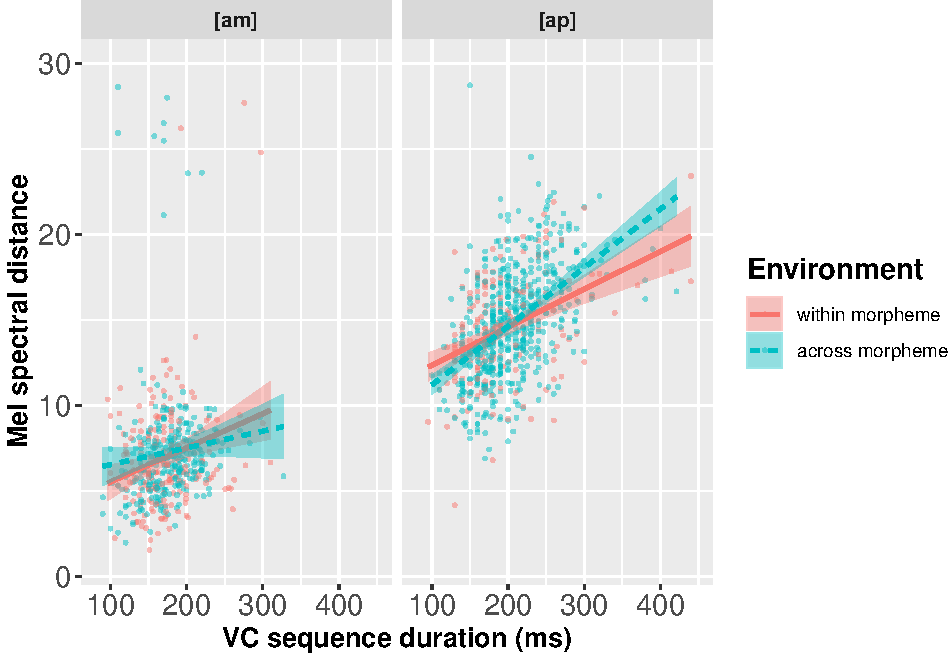
\includegraphics{3_ch3_results_files/figure-latex/adult-int-plot-1.pdf}
\caption{\label{fig:adult-int-plot}Coarticulation within VC sequence by sequence duration and morphological environment in adult speakers}
\end{figure}




\subsubsection{Adults}\label{adults}

For the adult model, the interaction between \textbf{Sequence duration}, \textbf{VC sequence}, and \textbf{Environment} suggests a difference in the relationship between the response variable - amount of coarticulation - and \textbf{Sequence duration} that differs by \textbf{Environment} and \textbf{VC sequence}. As Figure \ref{fig:adult-int-plot} demonstrates, this difference by \textbf{Environment} is apparent in the steepness of the slope for the `across morpheme' and `within morpheme' conditions for {[}am{]} and {[}ap{]}. To quantify this difference for the sequence {[}am{]}, the slopes of the two conditions were calculated. As the {[}am{]} panel in Figure \ref{fig:adult-int-plot} suggests, the slope for the `within morpheme' condition was steeper (2.14) than the slope for the `across morpheme' condition (2.06),\footnote{To reflect the data visualizations, these slopes were calculated on the beta coefficients before the coefficients were scaled by 100.} suggesting a different relationship between duration and coarticulation between the two word environments in adults.

Overall, the significance of the interaction \textbf{Sequence duration}, \textbf{VC sequence}, and \textbf{Environment} in adult speakers shows two important results: first, adults distinguish by word environment, both for {[}ap{]} versus {[}a\#p{]} sequences and {[}am{]} versus {[}a\#m{]} sequences. Second, complicating this finding, is the fact that adults distinguish between word environments differently depending upon the VC sequence. For {[}ap{]}, though adults coarticulate roughly equally across and within morphemes, the relationship between duration and coarticulation (longer duration equates to less coarticulation) is stronger in the `across morpheme' condition. For {[}am{]}, adults also distinguish between the two morphological environments by the relationship of VC duration and coarticulatory degree, but the effect of condition is reversed: the relationship between duration and coarticulation is stronger for the `within morpheme' condition.

Thus, returning to one part of the central research question - does adult coarticulation differ by word environment - we find that adults do coarticulate differently in the two word environments. However, despite these significant differences, there was nevertheless a positive relationship between duration and amount of coarticulation for all combinations of VC sequences and word environments. Adults consistently coarticulate less in longer-duration sequences. This result suggests that adult speakers may have one overarching articulatory plan for all environments and both VC sequences measured. The following section demonstrates how this relationship between duration and coarticulation may not be uniform between adults and children.

~

\subsubsection{Children}\label{children}

Turning to the child model, the significant interaction of \textbf{Sequence duration}, \textbf{VC sequence}, and \textbf{Environment} suggests that children do not coarticulate similarly in longer-duration sequences for all combinations of \textbf{Environment} and \textbf{VC sequence} (Figure \ref{fig:child-int-plot}). Specifically, for {[}ap{]} sequences that occur across morpheme boundaries, the negative slope indicates that children actually coarticulate \emph{more} in longer duration sequences. The positive slope for the within morpheme boundary condition suggests that children coarticulate less in longer-duration sequences, in line with all of the adult patterns. So, children coarticulate more between segments at morpheme boundaries in words inflected with the locative marker \emph{-pi} than between those same segments that occur within morphemes.

\begin{figure}[H]
\centering
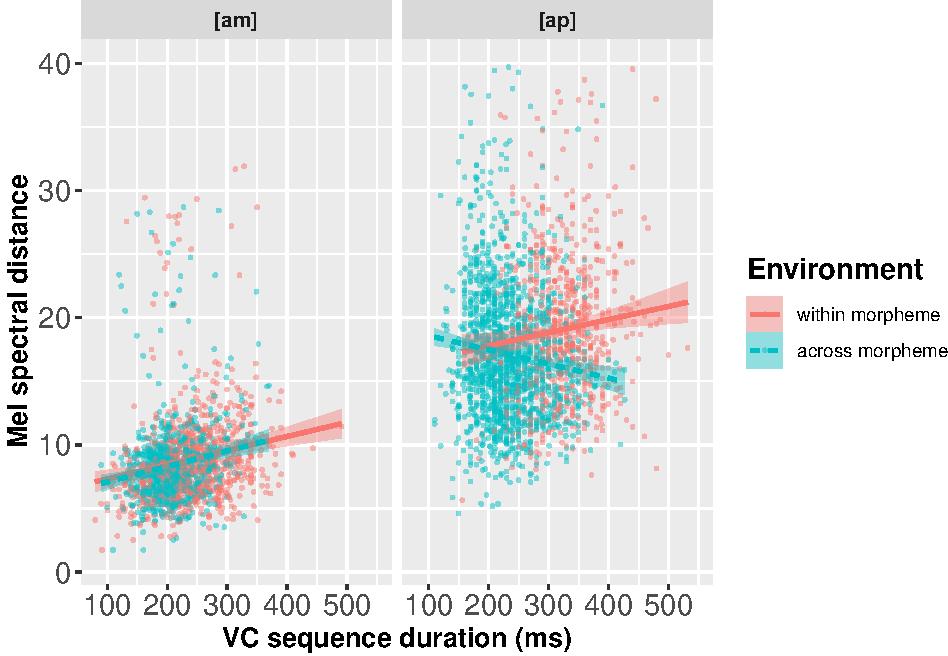
\includegraphics{3_ch3_results_files/figure-latex/child-int-plot-1.pdf}
\caption{\label{fig:child-int-plot}Coarticulation within VC sequence by sequence duration and morphological environment in all child speakers}
\end{figure}

\begin{figure}
\centering
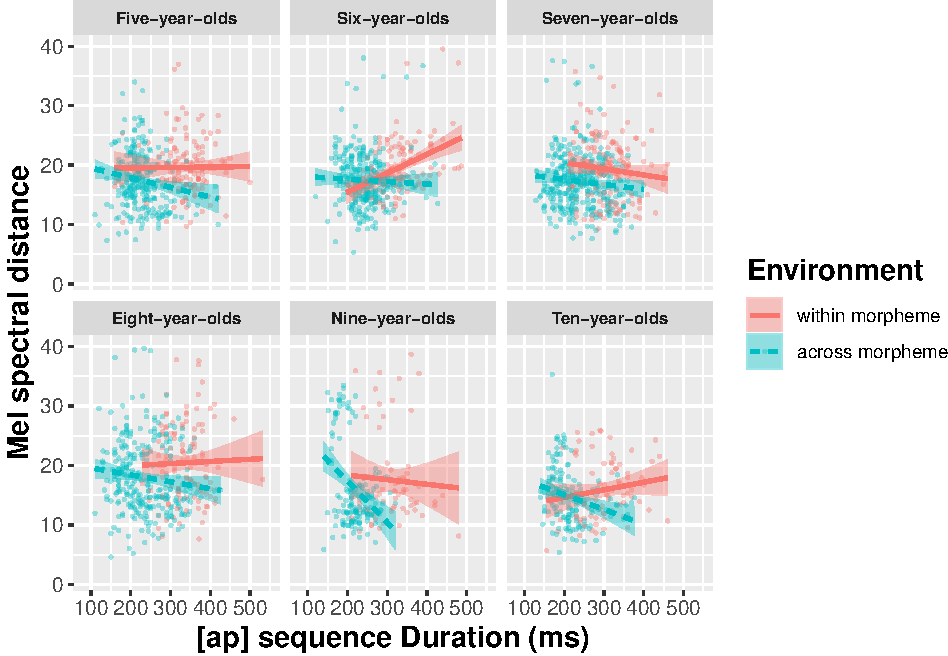
\includegraphics{3_ch3_results_files/figure-latex/child-facet-ap-1.pdf}
\caption{\label{fig:child-facet-ap}Coarticulation within {[}ap{]} by sequence duration, morphological environment, and age in child speakers}
\end{figure}

Note that this negative relationship between duration and coarticulation is counter to the positive relationship for every combination of VC sequence and word environment in adult speakers. Adults consistently coarticulate less in longer-duration sequences regardless of environment or VC sequence. The facet plot in Figure \ref{fig:child-facet-ap} plots this relationship between duration and coarticulation for {[}ap{]} for each age group (5-10 years) to ensure a consistent pattern across the groups. (Again the predictor \textbf{Age Group}, with the levels 5, 6, 7, 8, 9, and 10 years, did not improve upon the child model fit.) All age groups show the same negative relationship: the longer the {[}ap{]} sequence, the more the children coarticulate between {[}a{]} and {[}p{]} in the across morpheme condition.

\begin{figure}
\centering
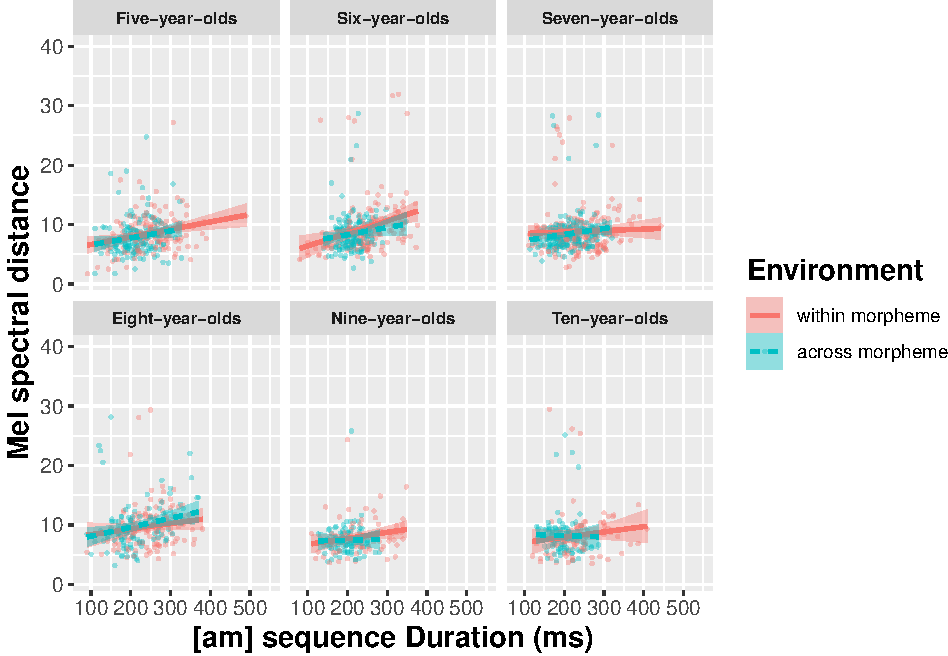
\includegraphics{3_ch3_results_files/figure-latex/child-facet-am-1.pdf}
\caption{\label{fig:child-facet-am}Coarticulation within {[}am{]} by sequence duration, morphological environment, and age in child speakers}
\end{figure}

The results for {[}am{]} in children demonstrate broadly similar results to the adult speakers: children coarticulate less between segments in longer-duration {[}am{]} sequences. The facet plot in Figure \ref{fig:child-facet-am} once again shows a similar effect for each age group. Given the between-subject variability that typically characterizes child speech, these patterns by environment are further broken apart by individual child for each age group (age 5-10) (Appendix \ref{app:app-E}) to ensure no large outliers with regards to the patterning by word environment. The results by are broadly similar across speakers.

~
~

{%
\subsection{Interim discussion}\label{interim-discussion}}

Comparing between the adult and child models, several preliminary conclusions can be made. First, responding to the original research question - do adults and children coarticulate differently within versus between morpheme boundaries - we find that both adults and children differentiate by morphological environment. However, they do so in different ways. Adults have a single plan for both environments, and even both VC sequences: adults coarticulate less in longer-duration sequences, and overall, they coarticulate less between {[}a{]} and {[}p{]} within morphemes than across morpheme boundaries. The stark difference between adults and children emerges in the {[}ap{]} sequence patterning. Children differentiate between morphological environments via the relationship between duration and coarticulation as they coarticulate more in longer-duration sequences across morpheme boundaries and coarticulate \emph{less} in longer-duration sequences within morphemes.

For words inflected with \emph{-man}, children show a similar pattern to adults, though children do not differentiate by environment coarticulatorily. Rather, across morpheme sequences are shorter in duration than within morpheme sequences for the children. On the basis of these results, two questions remain. First, why do children differentiate between environments via a combination of duration and coarticulation; specifically, why do children produce shorter duration VC sequences across morpheme boundaries and longer duration sequences within morphemes? Second, why do children coarticulate more in longer-duration {[}ap{]} sequences that cross morpheme boundaries (e.g.~\emph{llama-pi} `llama-\textsc{loc}')? All of the other combinations of morphological environment and VC sequence in the adults and children suggest that the speakers coarticulate less in longer-duration segments.

The finding that children produce shorter-duration VC sequences in the `across morpheme' condition than the `within morpheme' condition for {[}am{]} and {[}ap{]} could be explained by a confound in word size and morphological environment. Coarticulation for the `across morpheme' condition was, necessarily, measured across morphemes. However, to derive an across morpheme environment in Quechua, nouns are inflected with suffixes (e.g.~\emph{llama} `llama' -\textgreater{} \emph{llama-pi} `llama-\textsc{loc}'). As a result, almost all of the stimuli in the `across morpheme' condition are at least one syllable longer in length than the stimuli for the `within morpheme' condition. For example, coarticulation between {[}ap{]} was frequently measured within two syllable base roots (e.g.~\emph{llapa} `lightening' and \emph{llama} `llama'). However, for the `across morpheme' condition, {[}ap{]} coarticulation was frequently measured in three-syllable inflections of these nouns (e.g.~\emph{llapa-pi} `lightening-LOC' and \emph{llama-pi} `llama-\textsc{loc}'). Even for prosodically longer words where within morpheme coarticulation was measured, such as the three-syllable \emph{hampiri} `healer' and \emph{hatun mama} `grandmother', there were equivalent across morpheme stimuli that were one syllable longer (e.g.~\emph{hatun mama-mang} `grandmother-\textsc{all}').

~
~

\subsection{Compensatory shortening}\label{compensatory-shortening}

To explore the possibility that durational differences between the `across morpheme' and `within morpheme' conditions could be due to word length, an exploratory analysis was conducted. It was anticipated that sequence duration would shorten in words with more syllables, regardless of morphological context. This well-known tendency for segment durations to shorten in longer-duration/polysyllabic words is known as \textsc{Compensatory Shortening} (\citealt{harringtonRelationshipProsodicWeakening2015} \citealt{lehisteTimingUtterancesLinguistic1972}; \citealt{munhallCompensatoryShorteningMonosyllables1992}). To illustrate how this unfolds in the children's speech production for the current study, Figure \ref{fig:compshort-kids} plots VC sequence duration by the number of syllables for the children and Figure \ref{fig:compshort-adults} plots duration as a function of number of syllables for the adults. As the children's figure demonstrates, children's VC sequences are consistently shorter in words with more syllables, most notably between two- and three-syllable words. The same pattern is not apparent in the adult data: adults have fairly similar sequence lengths regardless of the number of syllables in the word (see Table \ref{tab:dur-by-syll-kids} for descriptive statistics of duration by word length in syllables for the children and Table \ref{tab:dur-by-syll-adults} for duration by word length results for the adults).

\begin{figure}
\centering
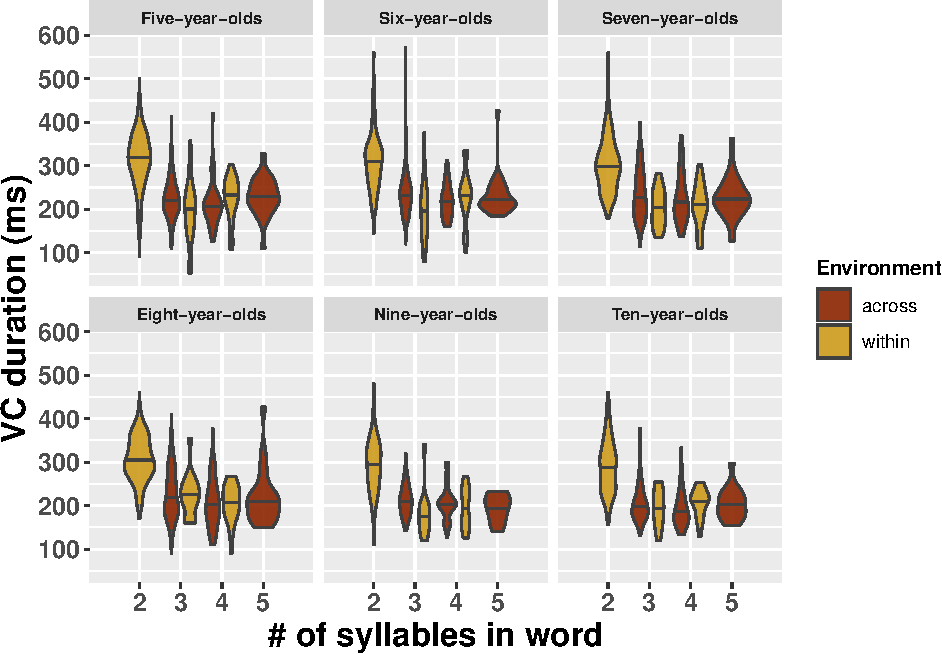
\includegraphics{3_ch3_results_files/figure-latex/compshort-kids-1.pdf}
\caption{\label{fig:compshort-kids}Sequence duration by word length and word environment: Children}
\end{figure}

\begin{figure}
\centering
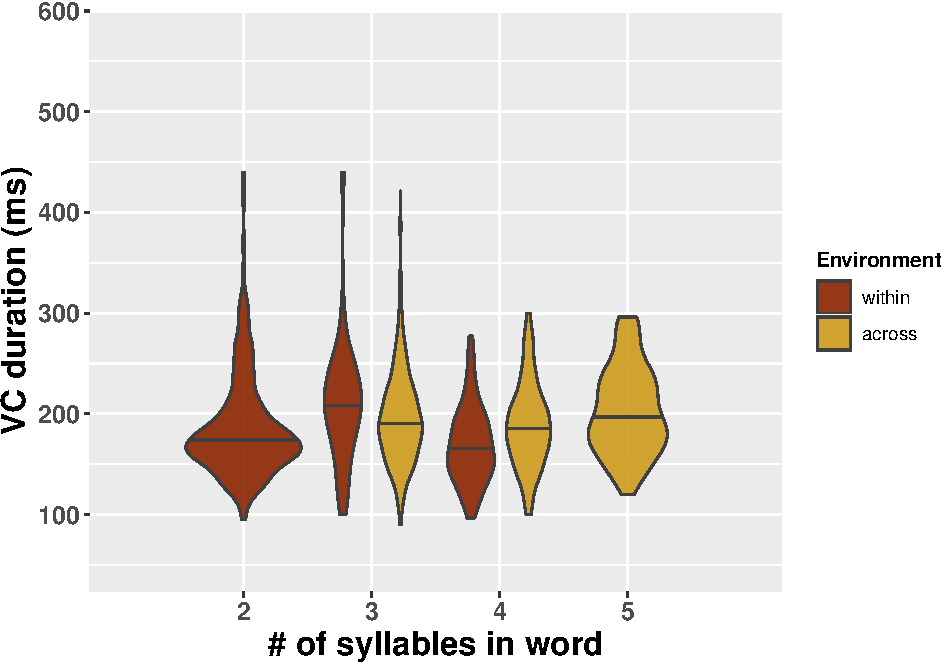
\includegraphics{3_ch3_results_files/figure-latex/compshort-adults-1.pdf}
\caption{\label{fig:compshort-adults}Sequence duration by word length and word environment: Adults}
\end{figure}

\begin{table}[H]

\caption{\label{tab:dur-by-syll-kids}Mean VC sequence duration by number of syllables in word for children}
\centering
\begin{tabular}[t]{lrrrr}
\toprule
\multicolumn{1}{c}{ } & \multicolumn{2}{c}{[am]} & \multicolumn{2}{c}{[ap]} \\
\cmidrule(l{3pt}r{3pt}){2-3} \cmidrule(l{3pt}r{3pt}){4-5}
Syllables & Duration (ms) & SD  & Duration (ms) & SD\\
\midrule
2 & 272.9 & 52 & 325.3 & 57\\
3 & 211.6 & 51 & 235.2 & 51\\
4 & 207.6 & 46 & 220.7 & 51\\
5 & 204.1 & 35 & 230.4 & 51\\
\bottomrule
\end{tabular}
\end{table}

\begin{table}[H]

\caption{\label{tab:dur-by-syll-adults}Mean VC sequence duration by number of syllables in word for adults}
\centering
\begin{tabular}[t]{lrrrr}
\toprule
\multicolumn{1}{c}{ } & \multicolumn{2}{c}{[am]} & \multicolumn{2}{c}{[ap]} \\
\cmidrule(l{3pt}r{3pt}){2-3} \cmidrule(l{3pt}r{3pt}){4-5}
Syllables & Duration (ms) & SD  & Duration (ms) & SD\\
\midrule
2 & 177.6 & 39 & 192.4 & 57\\
3 & 176.5 & 35 & 210.0 & 50\\
4 & 168.0 & 36 & 195.3 & 43\\
5 & 178.5 & 51 & 207.3 & 40\\
\bottomrule
\end{tabular}
\end{table}





To further explore the phenomenon of Compensatory Shortening in the children's speech, a linear mixed effects model was fit to predict the VC sequence duration in the children's speech (no skewed/non-negative predictors were included in the modelling so GLMMs were not necessary). Model fitting occurred as before in a forward-testing manner: the base model contained random effects of individual \textbf{Child} and \textbf{Word} (random slopes of Speaker by Word did not converge). Then, parameters were added in the following order: \textbf{Age} (5-10), \textbf{Number of Syllables} (2-5), \textbf{Environment} (across versus within), the interaction of \textbf{Number of Syllables} and \textbf{Environment}, and \textbf{VC sequence}. Only the predictors \textbf{Number of Syllables} and \textbf{VC sequence} improved baseline model fit (see Table \ref{tab:dursum} for model summary).

\begin{table}[!htbp] \centering 
  \caption{Model predicting VC duration: children} 
  \label{tab:dursum} 
\begin{tabular}{@{\extracolsep{5pt}}lc} 
\\[-1.8ex]\hline 
\hline \\[-1.8ex] 
 Intercept & 289.36$^{***}$ \\ 
  & (276.14, 302.58) \\ 
  & \\ 
 Three syllables & $-$79.68$^{***}$ \\ 
  & ($-$90.37, $-$68.99) \\ 
  & \\ 
 Four syllables & $-$93.38$^{***}$ \\ 
  & ($-$107.40, $-$79.37) \\ 
  & \\ 
 Five syllables & $-$87.01$^{***}$ \\ 
  & ($-$108.68, $-$65.34) \\ 
  & \\ 
 VC sequence:[ap] & 27.66$^{***}$ \\ 
  & (19.56, 35.77) \\ 
  & \\ 
\hline \\[-1.8ex] 
Observations & 3,877 \\ 
Log Likelihood & $-$20,122.98 \\ 
Akaike Inf. Crit. & 40,261.97 \\ 
Bayesian Inf. Crit. & 40,312.07 \\ 
\hline 
\hline \\[-1.8ex] 
\textit{Note:}  & \multicolumn{1}{r}{$^{*}$p$<$0.05; $^{**}$p$<$0.01; $^{***}$p$<$0.001} \\ 
\end{tabular} 
\end{table}

In the model summary, the positive beta coefficient for VC sequence with a reference level {[}am{]} indicates that the {[}ap{]} sequence was significantly longer than {[}am{]} sequences (as previous models demonstrated). Next, the negative beta coefficients for \textbf{Syllable Count} with a reference level of `2 syllables' indicated that VC sequence duration was approximately 80 ms shorter in three syllable words than two syllable (\(\beta\)=-79.68, t=-14.61, p\textless.001). Similarly, VC sequences were approximately 93 ms shorter in four syllable words than two syllable (\(\beta\)=-93.38, t=-13.06, p\textless.001) and 87 ms shorter in five syllable words than two syllable words (\(\beta\)=-87.01, t=-7.87, p\textless.001). The insignificance of \textbf{Environment} and child \textbf{Age} for the modelling suggests that that this relationship between duration and word length is independent of morphological environment and child age.

As these coefficients demonstrate, VC sequence decreases in larger words, with the largest differences between two- and three-syllable words. The diverse stimuli in the two- and three-syllable conditions (many different word types) suggest that this relationship by word length is relatively robust.

The only exception to the tendency to shorten sequences in larger words was that {[}ap{]} sequences are slightly longer in duration in 5-syllable words than 4-syllable words. However, in this exploratory analysis, the differences between the four and five syllable words were not tightly controlled: there were only two different five-syllable word stimuli: \emph{hatun mama-man} `grandmother-\textsc{all}'' and \emph{hatun mama-pi} `grandmother-\textsc{loc}'. We can only speculate that this relationship between sequence duration and number of syllables is strictly linear and would generalize to additional words with more syllables.

In conclusion, on the basis of this modeling, it is proposed that children may differentiate by morphological environment in their speech production. However, in Quechua, morphological structure is crossed with prosodic structure: complex words are always structurally longer than base forms. Regardless, children distinguish between morphological/prosodic environments primarily via the acoustic cue of \emph{duration}: in child Quechua, the duration of sequences is shorter in words with more syllables (Compensatory Shortening). This duration pattern by word length was not present in the adult speech, a finding that is explored in the Discussion.

~
~

\section{Discussion}

The experiment in this study employed a spectral measure of coarticulation to measure the coarticulatory patterns of adult and child Quechua speakers in two morphological environments. Two predictions were made for this experiment: 1) adult speakers would coarticulate less between two phones at a morpheme boundary than between the same phones within a morpheme boundary, and 2) child speakers would coarticulate more than adults between phones at morpheme boundaries. The reasoning behind these hypotheses was that  frequency ratios between suffixes, and between roots and suffixes, predict decompostability in adults (\citealt{hayCausesConsequencesWord2003}; \citealt{kempsProsodicCuesMorphological2005}; \citealt{ingoplagSuffixOrderingMorphological2009}). Adult speakers have more experience with language than children and have larger vocabularies \citep{lorgeEstimatingSizeVocabularies1963}. Consequently, adults may weigh the ratios of inflected to base forms in their lexicons differently. And children may structure relationships between base and suffixal forms differently as they age and their vocabularies grow. Moreover, children appear to coarticulate less as they age and gain more experience with words and segments \citep{noiraySpokenLanguageDevelopment2019}. A decrease in coarticulation suggests that phonological representations individuate into segment-sized units. For these reasons, it was predicted that adults might decompose words differently from children.

The results of this study appeared to confirm the first hypothesis. Adult speakers did, overall, coarticulate less across morpheme boundaries than within. This is to be expected because, if as previous studies suggest, speech production - coarticulation and duration - indexes lexical retrieval and composition (\citealt{choEffectsMorphemeBoundaries2001}; \citealt{kempsProsodicCuesMorphological2005}; \citealt{lee-kimMorphologicalEffectsDarkness2013}; \citealt{plagHomophonyMorphologyAcoustics2017}; \citealt{pluymaekersMorphologicalEffectsFine2010}; \citealt{songEffectsCoarticulationMorphological2013}; \citeyear{songDurationalCuesFricative2013}; \citealt{sugaharaDurationalCorrelatesEnglish2009}; \citealt{tomaschekHowAnticipatoryCoarticulation2019}). Specifically, the adult speakers tended to coarticulate less between phones in a VC sequence at a morpheme boundary than within a morpheme because adults are more likely to compose morphologically complex words from their component parts. Though decomposition is probabilistic (e.g. \citealt{hayCausesConsequencesWord2003}), overall, adults may be less likely to access morphologically complex words holistically. 

The results and conclusions of the second hypothesis proved far more complex, particularly given the interactions between degree of coarticulation and speaking rate/VC sequence duration. In slower speech, adult speakers coarticulated less, both across and within morphemes. This replicates known interactions between speaking rate (here instantiated as VC sequence duration) and coarticulation (\citealt{agwueleEffectSpeakingRate2008}; \citealt{matthiesVariationAnticipatoryCoarticulation2001}). In children, the same relationship between VC sequence duration and coarticulation appeared in the within-morpheme condition: within morphemes, children coarticulated less when they spoke slower. However, one primary difference between adults and children was that, in children, coarticulation did \textit{not} vary as a consequence of VC sequence duration in the across-morpheme condition. Of further interest was the finding that the children's VC sequence duration was reliably shorter in the across-morpheme condition than the within-morpheme condition. The following section interprets the duration finding from the children's data. 

\subsection{Compensatory shortening}

As suggested in the results section, one possible explanation for the shorter sequence duration in the across-morpheme condition for the children is the morphological structure of Quechua words. To construct morphologically complex words in this agglutinating language, additional suffixes must be appended to the root. As a result, almost all of the across-morpheme stimuli were approximately one syllable longer than the within-morpheme stimuli. It was suggested that the longer prosodic (and temporal) length of the stimuli in the across-morpheme condition caused children to shorten the duration of the phones in each of the stimuli items (or, variably, lengthen phone duration in the shorter, within-morpheme stimuli). This aligns with the well-known phenomenon of \textisc{compensatory shortening}, or segment duration shortening in longer-duration/polysyllabic lexical items (\citealt{harringtonRelationshipProsodicWeakening2015}; \citealt{lehisteTimingUtterancesLinguistic1972}; \citealt{munhallCompensatoryShorteningMonosyllables1992}).\footnote{The term compensatory shortening is also variably used in the literature to refer to shortening of stressed vowels compared to unstressed vowels in the context of polysyllabicity \citep{harringtonRelationshipProsodicWeakening2015}, or the shortening of stressed vowels in the context of unstressed vowels and consonants \citep{fowlerRelationshipCoarticulationCompensatory1981}.} This finding reinforces previous work on adult speech, as described in the literature review, that has demonstrated how roots have different variants in their bound and free forms \citep{kempsProsodicCuesMorphological2005}. One challenge in morphophonetics has been to identify the explanatory mechanisms behind morphologically-conditioned speech variation; at least in the current data, compensatory shortening could be one of these explanatory mechanisms. 

This relationship between-prosodic word size and segment duration is notable, but more interesting is the \textit{lack} of compensatory shortening in the adult speakers. While children demonstrated a trade-off in sequence duration and prosodic word size, adults were insensitive to word size. Yet previous findings on compensatory shortening came from adult populations. Why don't adults compensate for word size in their speech production as the children, even the eldest ten-year-olds, appear to?

There are several potential explanations for the difference in compensatory shortening between adults and children, some related to language experience and others reflecting sociolinguistics in Bolivia. First, adults speak faster than children \citep{leeAcousticsChildrenSpeech1999}, leading to more extreme phonetic reduction in their speech. Adult Quechua speakers may speak so much faster, and reduce so much more, than children that there could be insufficient freedom in their speech duration to differentiate sequence duration by prosodic word size. Children do not approximate adult-like speaking rates until early puberty (\citealt{leeAcousticsChildrenSpeech1999}; \citealt{smithRelationshipsDurationTemporal1992}). This increase in speaking rate is replicated in the present study, even in a tightly-controlled experimental setting, as the average VC sequence duration for the adult speakers was just 192 ms ($\sigma$=47) compared to 252 ms ($\sigma$=69) for the five-year-olds, 255 ms ($\sigma$=70), for the eight-year-olds, and 231 ms ($\sigma$=63) for the ten-year-olds. 

Speakers reduce significantly more in fast speech compared to slower, controlled speech. In fast speech, the vowel space is smaller and more centralized (\citealt{fourakisTempoStressVowel1991}; \citealt{tsaoEffectIntertalkerSpeech2006}) - which may compromise contrasts \citep{koopmans-vanbeinumVowelContrastReduction1980}, increase coarticulation between phones (\citealt{agwueleEffectSpeakingRate2008}; \citealt{matthiesVariationAnticipatoryCoarticulation2001}), and cause the omission of entire segments or syllables \citep{johnsonMassiveReductionConversational2004}. For the current study, the durational data summarized in the previous paragraph suggest that all adult speech, regardless of prosodic or morphological structure, is maximally fast and reduced.  

Though there is little work on the phonetics of highly morphologically complex languages, the author can anecdotally attest to how speaking rate interplays with word structure in Quechua. Just as the orthographic forms of English words rarely correspond to their phonetic realization in fast, spontaneous speech, spoken words in Quechua deviate from their citation form. In Quechua, this is especially true with large words that contain numerous suffixes, where the most extreme reduction can be seen. In Quechua, the further a suffix is found from the root, the \textit{more} likely it is to be reduced (shorter in duration, omission of segments/syllables). The explanation for this is partially aerodynamic (e.g. airflow). But there are also likely perceptual and information-theoretic explanations. When suffixes are highly reduced compared to stems, speakers can more easily demarcate between suffixes and roots, and identify word boundaries \citep{zinglerReductionFusionGrammaticalization2018}. Furthermore, word meanings are likely increasingly predictable as additional suffixes are added and the available semantic space of the word narrows.\footnote{For English, however, Plag and Baayen (2009) found that those suffixes farthest from the stem are also the most productive and available for use in novel environments.} Variability in the phonetic realization of English morphology (e.g. plurals) is dependent upon the predictability of plurality given the sentence frame \citep{cohenProbabilisticReductionProbabilistic2014}, so it is possible that speakers likewise make probability calculations over multiple suffixes. Much more work is needed to understand probabilistic reduction based on word structure. However, overall, one explanation for adults' lack of compensatory lengthening is their speaking rate and phonetic reduction.

A second explanation for the lack of compensatory shortening in adults may be that the adults are more dominant in Quechua than the children. This means that the adults may speak faster and, again, may be unable to differentiate prosodic structure via duration. Recent changes in Bolivia's educational policy, as well as the country's general sociolinguistic situation, may have led to adults' increased fluency. Bilingual education in Bolivia became mandatory in 1994 and has, in theory, been relatively widespread since the early 2000s \citep{bensonBilingualSchoolingMozambique2004}. This means more children, especially indigenous students and young girls, are attending and completing more schooling than ever before \citep{hornbergerMultilingualEducationPolicy2009}. 

In practice, however, bilingual education often takes the form of Spanish-only classrooms. In Quechua-speaking areas, many trained teachers do not speak Quechua fluently or are not provided with teaching materials and textbooks written in Quechua. The result - students completing more schooling but instructed in Spanish - has been rapid language shift \citep{hornbergerLanguageRevitalisationAndes1996}. This has been apparent even in the last decade, as the first generation of women educated in this system are now raising their children using both Quechua and Spanish, instead of monolingual Quechua, in an increasingly Spanish-dominant environment. 

These sociolinguistic dynamics could manifest in the present sample as the adult female participants (many of whom are mothers) may be more Quechua-dominant than some of the children in the sample. Though the adult females who participated in the study were only, on average, 13 years older than the eldest children (adult $\mu$\textsubscript{age}=23 years; $\sigma$=5.46 years), and all adults and children identified as bilingual Quechua-Spanish speakers, their language practices may reflect the recent changes in educational policy. It is also important to note that all of the children in the sample attended school, in Spanish, for 3-4 hours per day. However, only one of the adult females was still attending school (taught in Spanish). This difference could also explain usage patterns between the age groups.

If the adult females were more Quechua-dominant, or used Quechua more frequently, they would speak faster, more fluently, and could reduce more, as described above. Thus, although the adult speakers in this study undoubtedly did speak faster than the children for speech maturation reasons - it takes time and practice to master the articulatory speed of an adult \citep{leeAcousticsChildrenSpeech1999} - the adults may also have spoken Quechua faster, and thus failed to compensate for prosodic structure to the degree that the children did, because they use Quechua more frequently. This proposal may not entirely explain the differences in compensatory shortening between the adult and child Quechua speakers - previous studies on compensatory shortening (\citealt{lehisteTimingUtterancesLinguistic1972}; \citealt{munhallCompensatoryShorteningMonosyllables1992}) reported on highly-fluent, monolingual adult speakers who \textit{did} compensate for prosodic structure - but it is one explanation for the differences observed between age groups in the present work. 

While this study did not report participants' bilingual language dominance, all speakers identified as Quechua-Spanish bilinguals and reported using both languages.\footnote{Computation of the children's language dominance is underway using naturalistic recordings of the children's daily language usage. This method skirts the issue of self-reported usage.} The decision not to conduct a traditional language usage survey was made for several reasons. Traditional measures of self-reported bilingual dominance, such as the bilingual language profile \citep{birdsonBilingualLanguageProfile2012}, often rely on participant literacy or familiarity and comfort with written behavioral research surveys. Also, the traditional stigmatization of indigenous languages in Bolivia may render self-reports of language dominance unreliable. Nevertheless, one potential difference between the adults and children could be their Quechua language usage or dominance. 



\subsection{Do children distinguish between morphological environments in their speech production?}

The original research question in this study asked if adults and children coarticulated differently across versus within morpheme boundaries. As the discussion of compensatory shortening outlined, children appear to distinguish by morphological environment, suggesting that they decompose words. However, this could be a consequence of prosodic structure, which is correlated with morphological structure in Quechua. The different temporal and coarticulatory patterns seen in the across- and within-morpheme conditions could reflect morphological structure and lexical access, or the patterns could reflect prosodic structure. Children may modulate their speech temporally to demarcate between morphological environments - faster segments across morphemes and slower segments within. Or, as compensatory shortening suggests, children may shorten the duration of VC sequences in prosodically longer words. 

One way to evaluate these two explanations is to control for prosodic structure by measuring duration and coarticulation across morphemes versus within morphemes, but always in words of the same length (in number of syllables). This is made more difficult in Quechua because the language has canonical penultimate stress: even if duration/coarticulation were measured between [am] in a three-syllable within-morpheme stimulus (e.g. ll\textbf{a}.\textsf{'}\textbf{m}a.-man `llama-\textsc{all}'), and a corresponding three-syllable across-morpheme stimulus (e.g. pa.\textsf{'}p\textbf{a}.-\textbf{m}an `potato-\textsc{all}'), the stress would not be controlled. In other words, any differences in duration/coarticulation patterns between the across-morpheme and within-morpheme stimuli could be attributable to known acoustic correlates of stress, and might not reflect morphological \textit{or} prosodic structure. This issue reflects some recent acknowledgements in morphophonetics that it may be nearly impossible to design studies that perfectly isolate morphological effects from the plethora of other correlated variables (\citealt{strycharczukPhoneticDetailPhonetic2019}, cf. \citealt{seyfarthAcousticDifferencesMorphologicallydistinct2018}). 

In the current dataset there are three lexical items that control for prosody (and thus stress) and allow us to tease apart the prosodic versus morphological explanations for the children's patterns. Specifically, there are three four-syllable stimuli - two across morpheme (\textit{imi\textsf{'}ll\textbf{a-m}an} `girl-\textsc{all}' and \textit{juk'u\textsf{'}ch\textbf{a-m}an
} `mouse-\textsc{all}') and one within morpheme (\textit{hatun\textsf{'}m\textbf{am}a}) - where the [a] of [am] falls in stressed position. In the following exploratory analysis, the duration of [am] and the coarticulation between [a] and [m] were measured for all of the children and adults. Results are listed in tables \ref{tab:4syll-table-dur} and \ref{tab:4syll-table-coartic}. 

 \begin{table}[H]
\caption{\label{tab:4syll-table-dur}Mean duration of [am] across and within morphemes in prosodically-controlled stimuli}
\centering
\begin{tabular}[t]{lrrrr}
\toprule
\multicolumn{1}{c}{ } & \multicolumn{2}{c}{Across boundary} & \multicolumn{2}{c}{Within boundary} \\
\cmidrule(l{3pt}r{3pt}){2-3} \cmidrule(l{3pt}r{3pt}){4-5}
Age & Duration  & SD  & Duration & SD\\
\midrule
 5 & 193.3(ms)  & 32 & 245.7 & 30 \\
 6 & 199.0  & 25 & 242.9  & 50 \\
 7 & 188.8  & 34 & 229.8  & 36 \\
 8 & 205.3  & 49 & 225.2  & 30 \\
 9 & 189.4  & 37 & 226.4  & 32 \\
 10 & 170.9 & 26 & 216.6 & 17 \\
adult & 165.4 & 30 & 230.6 & 33 \\
\bottomrule
\end{tabular}
\end{table}

 \begin{table}[H]
\caption{\label{tab:4syll-table-coartic}Mean spectral distance between [a] and [m] across and within morphemes in prosodically-controlled stimuli}
\centering
\begin{tabular}[t]{lrrrr}
\toprule
\multicolumn{1}{c}{ } & \multicolumn{2}{c}{Across boundary} & \multicolumn{2}{c}{Within boundary} \\
\cmidrule(l{3pt}r{3pt}){2-3} \cmidrule(l{3pt}r{3pt}){4-5}
Age & Spectral Distance  & SD  & Spectral Distance & SD\\
\midrule
 5 & 7.34 & 2.52 & 8.49 & 2.45 \\
 6 &  9.78 & 5.84 & 9.51 & 5.39 \\
 7 & 7.85 & 1.30 & 8.82 & 5.05 \\
 8 & 9.61 & 4.00 & 8.89 & 3.37 \\
 9 & 7.62 & 1.88 & 6.63 & 2.15 \\
 10 &  8.34 & 1.57 & 8.29 & 4.66\\
adult & 8.90 & 4.17 & 5.48 & 1.20 \\
\bottomrule
\end{tabular}
\end{table}


 
As the results demonstrate, both the children and adults have shorter [am] sequences in the across-morpheme condition (stimuli \textit{imilla-man} and \textit{juk'ucha-man}). The duration of [am] also decreases with age, as the adults speak fastest. Thus, when controlling for prosody, it appears that children do pattern like the adults and may distinguish by morphological environment using durational cues. However, for coarticulation, the results differ between adults and children. While the children do not appear to distinguish greatly between morphological environments, coarticulating roughly equally in the two environments regardless of age, the adults distinguish between the two areas. As anticipated from previous work (e.g. \citealt{choEffectsMorphemeBoundaries2001}), the spectral distance between [a] and [m] is greater in the across-morpheme stimuli (\textit{imill\textbf{a-m}ang} and \textit{juk'uch\textbf{a-m}an} than the within-morpheme stimulus (\textit{hatunm\textbf{am}a}). Unlike the durational results, the exploratory coarticulation results suggest that adults, but not children, distinguish between the the morphological environments. 

These data are too sparse to make definitive conclusions; only three distinct lexical items were tested. Concerning the central research question - do children distinguish between morphological environments - the exploratory analysis gave conflicting results: children distinguish between environments like adults durationally, but not coarticulatorily. However, the exploratory analysis does suggest that children's compensatory lengthening is likely morphological in nature, not prosodic, since the [am] was shorter in duration in the across-morpheme condition in the four-syllable stimuli. 
 
Thus, using a combination of coarticulatory and temporal cues in their production, children appear to distinguish between across-morpheme and within-morpheme stimuli. But, in most of the current stimuli, morphological environment is correlated with prosodic environment (to derive morpheme boundaries, extra syllables must be added to roots). It therefore remains unclear if children's different speech patterns across the two morphological environments reflect prosodic planning, lexical planning, or both. 

Future work, ideally on languages with different and complex morphological structures, is needed to further explore the relationships between children's speech production and word structure. Going forward, researchers may also benefit from the use of articulatory measures, in addition to acoustic measures, to explore the relationships between coarticulation and morphological structure in children. Given the logistics of ultrasound imaging, and the limitations of fieldwork, the current study was not able to collect articulatory data, which would otherwise be a valuable addition.

This study was unable to control for, or examine the effect of, lexical frequency of the base or inflected forms. This is unfortunate because much variability in morphological parsing, and morphophonetics, is attributable to lexical frequency \citep{seyfarthAcousticDifferencesMorphologicallydistinct2018} or frequency ratios between stems and suffixes (\citealt{hayCausesConsequencesWord2003}; \citealt{ingoplagSuffixOrderingMorphological2009}). At this time, however, it is not possible to reliably calculate lexical frequency statistics for Quechua, and indeed for most of the world's languages. A large, naturalistic corpus of child and adult Bolivian Quechua has recently been collected \citep{cychoszCychoszHomeBankCorpus2018}, but it will be years before it is sufficiently transcribed to calculate lexical statistics. In the mean time, researchers interested in the morphophonetics of underdocumented languages could possibly use age of acquisition as a proxy for word frequency \citep{morrisonAgeAcquisitionNot1992} and this may a promising methodological approach should researchers hope to include additional under-documented languages in the study of morphophonetics.\footnote{The author found that obtaining age of acquisition norms was not possible for the current study because the Quechua-speaking adults were relatively unfamiliar with behavioral research and the methods that would have been required to solicit age of acquisition information.} 

\section{Conclusion}

The primary goal of this study was to compute coarticulation in adult and child Quechua speakers in two morphological environments: within morphemes and across morpheme boundaries. Results showed that, using a combination of coarticulatory and temporal cues, adults distinguished between the two morphological environments in their speech production. This replicated known speech production patterns by word environment but in an understudied, morphologically complex language. The children showed increased prosodic sensitivity where the adults did not: children shortened the duration of sequences in prosodically longer words, which also happened to be morphologically complex. It was suggested that the difference between adults and children could be attributable to adults' faster speaking rate and increased practice with Quechua. An exploratory analysis isolating prosodic effects from morphological was conducted on a subset of the original data. This analysis suggested that children's speech patterns may be reflecting morphological structure, though future work is needed to determine the level of children's speech planning: prosodic, morphological, or both. Overall, these analyses have demonstrated some of the complexities that arise in morphophonetic patterning and speech development, and the importance of extending recent studies in this sub-domain of phonetics to languages with vastly different word structures and speakers with different language experiences. 

\section*{Declaration of interest}
The author has no competing interests to report. 

\section*{Acknowledgements}


\theendnotes

\bibliography{references}

\appendix
\section{South Bolivian Quechua Consonant Inventory}\label{app:app-A}

\begin{table}

\centering
	\begin{tabular}{l|c|c|c|c|c|c|c|c|c|c}
			    & 
				\multicolumn{1}{c|}{\footnotesize{Bilabial}} &					% Bilabial
				\multicolumn{1}{c|}{\footnotesize{Dental}} & 					% Dental
				\multicolumn{1}{c|}{\footnotesize{Postalveolar}} & 		% Post-alveolar
		       \multicolumn{1}{c|}{\footnotesize{Palatal}} & 		
		       % palatal
				\multicolumn{1}{c|}{\footnotesize{Velar}} & 					% Velar
				\multicolumn{1}{c|}{\footnotesize{Uvular}} & 					% Uvular
				\multicolumn{1}{c}{\footnotesize{Glottal}}  \\					% Glottal

			\hline Plosive &  % Plosive
			        \textipa{p}  & % bilabial
			        \textipa{t}	&	% Dental
					\textipa{\textteshlig}	& % Post-alveolar
					\Blankcell &	% Palatal
				    \textipa{k} &	% Velar
			      	\textipa{q} &	% Uvular
				   \Blankcell \\	% Glottal
				   
		     \hline Aspirated &  % Plosive
			        \textipa{p}\textsuperscript{h}  & % bilabial
			        \textipa{t}\textsuperscript{h}	&	% Dental
					\textipa{\textteshlig}\textsuperscript{h}	& % Post-alveolar
					\Blankcell &	% Palatal
				    \textipa{k}\textsuperscript{h} &	% Velar
			      	\textipa{q}\textsuperscript{h} &	% Uvular
				   \Blankcell \\	% Glottal
				   
			 \hline Ejective &  % Plosive
			        \textipa{p}'  & % bilabial
			        \textipa{t}'	&	% Dental
					\textipa{\textteshlig}'	& % Post-alveolar
					\Blankcell &	% Palatal
				    \textipa{k}' &	% Velar
			      	\textipa{q}' &	% Uvular
				   \Blankcell \\	% Glottal

			\hline Nasal & 	% Nasal
				\textipa{m} & % Bilabial
				\textipa{n}	& % Dental
			    \Blankcell & % Post-alveolar
			    \textltailn &	% Palatal
				\Blankcell  & % Velar
				\Blankcell	& % Uvular
				\Blankcell \\% Glottal

			\hline Fricative &  % Fricative
				\Blankcell &	% Labial
				\ipa{s} & % Dental
			    \Blankcell	& % Post-alveolar
			    \Blankcell &	% Palatal
				\Blankcell	& % Velar
				\Blankcell	& % Uvular
				\textipa{h}	\\ % Glottal
				
			\hline Tap & % Tap 
				\Blankcell	& % Bilabial
				\textfishhookr & % Dental
				\Blankcell	& % Post-alveolar
				\Blankcell &	% Palatal
				\BlankCell 	& % Velar
				\Blankcell	& % Uvular
				\BlankCell  \\ % Glottal

			\hline Approximant & % Approx.
				\textipa{w} & % Bilabial
				\BlankCell	& % Dental
				\textturny 	& % Post-alveolar
				\textipa{j} &	% Palatal
				\Blankcell & % Velar
				\Blankcell & % Uvular
				\BlankCell \\ % Glottal

			\hline Lateral & % Lateral
				  \BlankCell  & % Bilabial
			      \textipa{l} & % Dental
				  \Blankcell  & % Post-alveolar
				  \Blankcell &	% Palatal
				 \BlankCell &	% Velar
				 \BlankCell  & % Uvular
				 \BlankCell	\\ % Glottal
		\end{tabular}
		\end{table}


\section{Stimuli used in real word repetition tasks}\label{app:app-B}
\begin{table}

\centering
\begin{tabular}{c | c} 
\hline
Real word* & Translation  \\
\hline

\footnotesize{\textsf{'}warmi} & `woman' \textit{training trial}\\
\footnotesize{\textsf{'}wasi} & `house' \textit{training trial} \\
\footnotesize{\textsf{'}qhari} & `man' \textit{training trial}\\
\footnotesize{\textsf{'}chita} & `sheep' \\
\footnotesize{\textsf{'}p'esqo} & `bird' \\
\footnotesize{ju\textsf{'}k'ucha} & `mouse' \\
\footnotesize{\textsf{'}waka} & `cow' \\
\footnotesize{\textsf{'}wallpa} & `chicken' \\
\footnotesize{\textsf{'}mama} & `mom' \\
\footnotesize{\textsf{'}papa} & `potato' \\
\footnotesize{\textsf{'}t'ika} & `flower' \\
\footnotesize{\textsf{'}llama} & `llama' \\
\footnotesize{\textsf{'}cuca} & `coca (leaves)' \\
\footnotesize{u\textsf{'}hut'a} & `sandal' \\
\footnotesize{ham\textsf{'}piri} & `healer' \\
\footnotesize{i\textsf{'}milla} & `girl' \\
\footnotesize{\textsf{'}llapa} & `lightening' \\
\footnotesize{\textsf{'}api} & `corn/citrus drink' \\
\footnotesize{\textsf{'}ch'ulu} & `hat' \\
\footnotesize{\textsf{'}punku} & `door' \\
\footnotesize{\textsf{'}thapa} & `nest' \\
\footnotesize{\textsf{'}punchu} & `poncho' \\
\footnotesize{\textsf{'}pampa} & `prairie' \\
\footnotesize{\textsf{'}sunkha} & `beard' \\
\footnotesize{hatun\textsf{'}mama} & `grandma' \\
\footnotesize{\textsf{'}wawa} & `baby/child' \\
\footnotesize{\textsf{'}runtu} & `egg' \\
\footnotesize{\textsf{'}qolqe} & `money' \\
\footnotesize{\textsf{'}q'apa} & `palm of hand' \\
\footnotesize{\textsf{'}alqo} & `dog' \\
\footnotesize{\textsf{'}q'epi} & `bundle' \\
 \hline

\end{tabular}\par
\smallskip
* For the real words, \textsf{'} indicates stress, ' indicates ejective
\end{table}

\section{Real word repetition stimuli to elicit [am]}\label{app:app-C}

\begin{table}\small

\centering
\begin{tabular}{c | c| c} 
\hline
Real word* & Translation & \thead{Morpheme environment\textsuperscript{\textdagger}}\\
\hline

\footnotesize{chi\textsf{'}t\textbf{a-m}an} & 'sheep-\textsc{all}' & across \\
\footnotesize{cu\textsf{'}c\textbf{a-m}an} & 'coca (leaves)-\textsc{all}' & across \\
\footnotesize{hatunma\textsf{'}m\textbf{a-m}an} & 'grandma-\textsc{all}' & across \\
\footnotesize{imi\textsf{'}ll\textbf{a-m}an} & 'girl-\textsc{all}' & across \\
\footnotesize{juk'u\textsf{'}ch\textbf{a-m}an} & 'mouse-\textsc{all}' & across \\
\footnotesize{lla\textsf{'}m\textbf{a-m}an} & 'llama-\textsc{all}' & across \\
\footnotesize{lla\textsf{'}p\textbf{a-m}an} & 'lightening-\textsc{all}' & across \\
\footnotesize{ma\textsf{'}m\textbf{a-m}an} & 'mom-\textsc{all}' & across \\
\footnotesize{pam\textsf{'}p\textbf{a-m}an} & 'prairie-\textsc{all}' & across \\
\footnotesize{pa\textsf{'}p\textbf{a-m}an} & 'potato-\textsc{all}' & across \\
\footnotesize{q'a\textsf{'}p\textbf{a-m}an} & 'palm of hand-\textsc{all}' & across \\
\footnotesize{sun\textsf{'}kh\textbf{a-m}an} & 'beard-\textsc{all}' & across \\
\footnotesize{t'i\textsf{'}k\textbf{a-m}an} & 'flower-\textsc{all}' & across \\
\footnotesize{tha\textsf{'}p\textbf{a-m}an} & 'nest-\textsc{all}' & across \\
\footnotesize{wa\textsf{'}k\textbf{a-m}an} & 'cow-\textsc{all}' & across \\
\footnotesize{wall\textsf{'}p\textbf{a-m}an} & 'chicken-\textsc{all}' & across \\
\footnotesize{wa\textsf{'}w\textbf{a-m}an} & 'baby/child-\textsc{all}' & across \\

\hline

\footnotesize{\textsf{'}m\textbf{am}a} & 'mom' & within \\
\footnotesize{\textsf{'}ll\textbf{am}a} & 'llama' & within \\
\footnotesize{h\textbf{am}\textsf{'}piri} & 'healer' & within \\
\footnotesize{h\textbf{am}pi\textsf{'}ri-pi} & 'healer-\textsc{loc}' & within \\
\footnotesize{\textsf{'}p\textbf{am}pa} & 'prairie' & within \\
\footnotesize{hatun\textsf{'}m\textbf{am}a} & 'grandma' & within \\

 \hline
\end{tabular}\par
\smallskip
* ' indicates stress, \textsf{'} indicates ejective\par
\smallskip
\end{table}

\section{Model predicting coarticulation in children and adults}\label{app:app-D}

\begin{table}
\AtBeginEnvironment{tabular}{\singlespacing}
\begin{center}
\begin{threeparttable}
\begin{tabular}{lllllll}
\toprule
 & \multicolumn{1}{c}{estimate} & \multicolumn{1}{c}{S.E.} & \multicolumn{1}{c}{z.statistic} & \multicolumn{1}{c}{p.value} & \multicolumn{1}{c}{95\% CI} \\
\midrule
\thead{Intercept} & 2.14 & 0.04 & 59.61 & 0.00 & 2.21,2.07\\
\thead{Sequence duration scaled} & 0.00 & 0.00 & 3.65 & 0.00 & 0,0\\
\thead{VC sequenceap} & 0.73 & 0.05 & 16.20 & 0.00 & 0.82,0.64 \\
\thead{Environment:across morpheme} & -0.05 & 0.07 & -0.67 & 0.50 & 0.09,-0.19 \\
\thead{Sequence duration*VC sequence:ap} & 0.02 & 0.03 & 0.57 & 0.57 & 0.09,-0.05 \\
\thead{Sequence duration*\\VC sequence:ap} & 0.00 & 0.00 & -0.63 & 0.53 & 0,0 \\
\thead{Sequence duration*\\Age:adult} & 0.00 & 0.00 & 2.66 & 0.01 & 0,0 \\
\thead{VC sequence:ap*Age:adult} & -0.10 & 0.06 & -1.71 & 0.09 & 0.01,-0.21 \\
\thead{Sequence duration*\\Environment:across morpheme} & 0.00 & 0.00 & 2.37 & 0.02 & 0,0 \\
\thead{VC sequence:ap*\\Environment:across morpheme} & -0.06 & 0.05 & -1.17 & 0.24 & 0.04,-0.17 \\
\thead{Age:adult*\\Environment:across morpheme} & -0.09 & 0.05 & -1.74 & 0.08 & 0.01,-0.2 \\
\thead{Sequence duration*\\VC sequence:ap*Age:adult} & 0.00 & 0.00 & -1.25 & 0.21 & 0,0 \\
\thead{Sequence duration scaled*\\VC sequence:ap:Environmentacross morpheme} & 0.00 & 0.00 & -2.25 & 0.02 & 0,0 \\
\thead{Sequence duration*Age:adult*\\Environment:across morpheme} & 0.00 & 0.00 & -3.36 & 0.00 & 0,0 \\
\thead{VC sequence:ap*A\\ge:adult*Environment:across morpheme} & 0.16 & 0.07 & 2.31 & 0.02 & 0.29,0.02 \\
\thead{Sequence duration*\\VC sequence:ap*Age:adult*Environment:across morpheme} & 0.00 & 0.00 & 3.44 & 0.00 & 0,0 \\
\bottomrule
\end{tabular}
\end{threeparttable}
\end{center}
\end{table}

\section{Coarticulation by sequence duration, word, and morphological environment in children}\label{app:app-E}

\begin{figure}
\centering
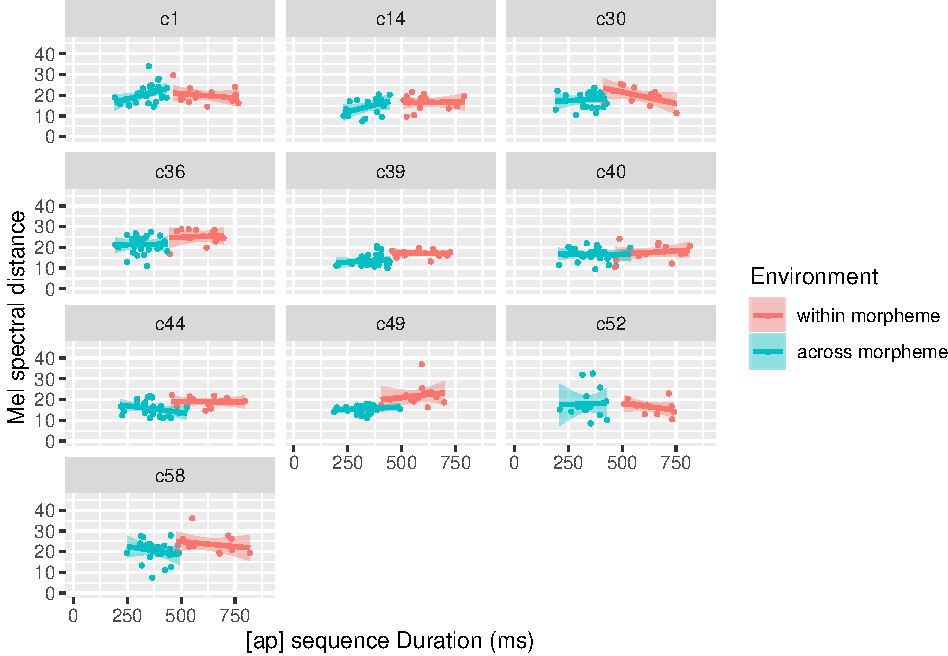
\includegraphics{3_ch3_results_files/figure-latex/five-facet-ap-1.pdf}
\caption{\label{fig:five-facet-ap}Coarticulation by {[}ap{]} duration, word, and morphological environment in five-year-old children}
\end{figure}

\begin{figure}
\centering
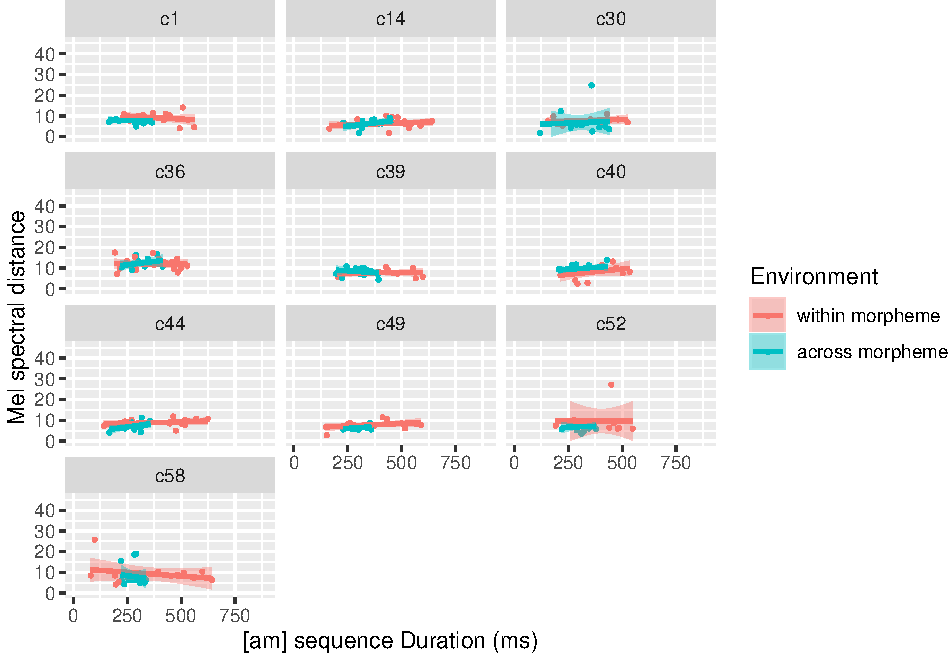
\includegraphics{3_ch3_results_files/figure-latex/five-facet-am-1.pdf}
\caption{\label{fig:five-facet-am}Coarticulation by {[}am{]} duration, word, and morphological environment in five-year-old children}
\end{figure}

\begin{figure}
\centering
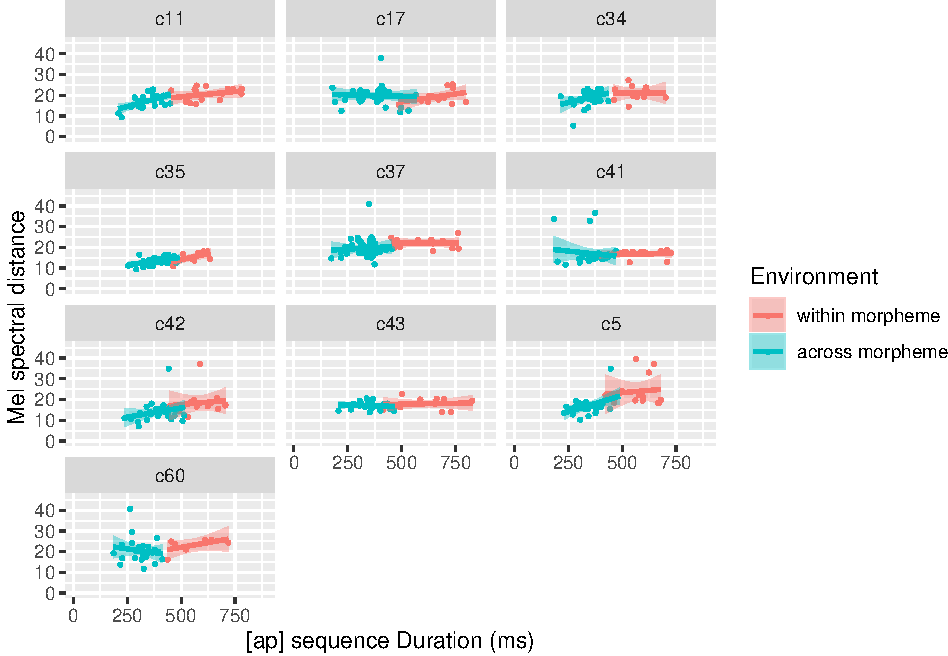
\includegraphics{3_ch3_results_files/figure-latex/six-facet-ap-1.pdf}
\caption{\label{fig:six-facet-ap}Coarticulation by {[}ap{]} duration, word, and morphological environment in six-year-old children}
\end{figure}

\begin{figure}
\centering
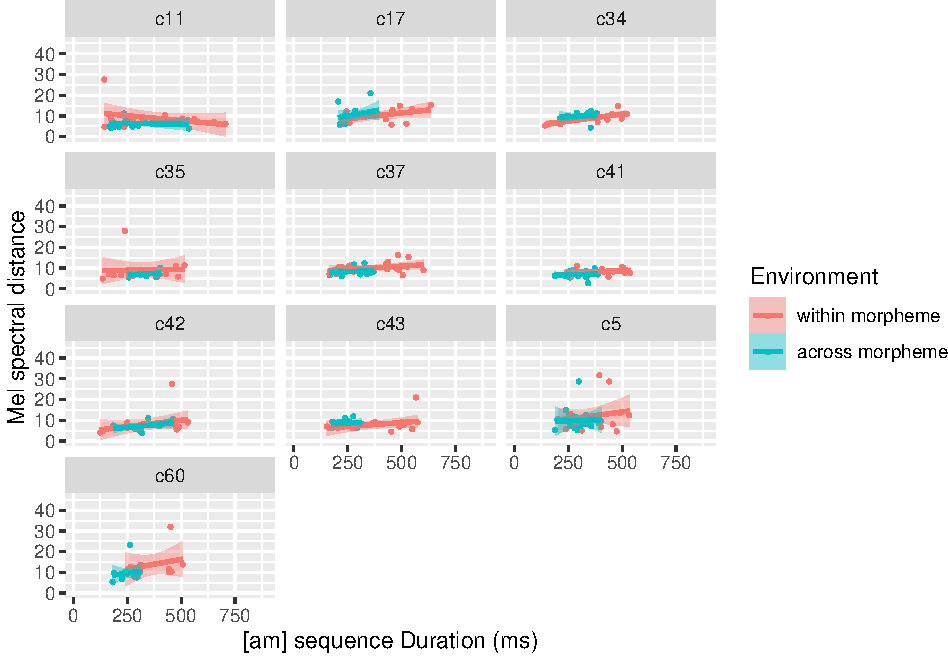
\includegraphics{3_ch3_results_files/figure-latex/six-facet-am-1.pdf}
\caption{\label{fig:six-facet-am}Coarticulation by {[}am{]} duration, word, and morphological environment in six-year-old children}
\end{figure}

\begin{figure}
\centering
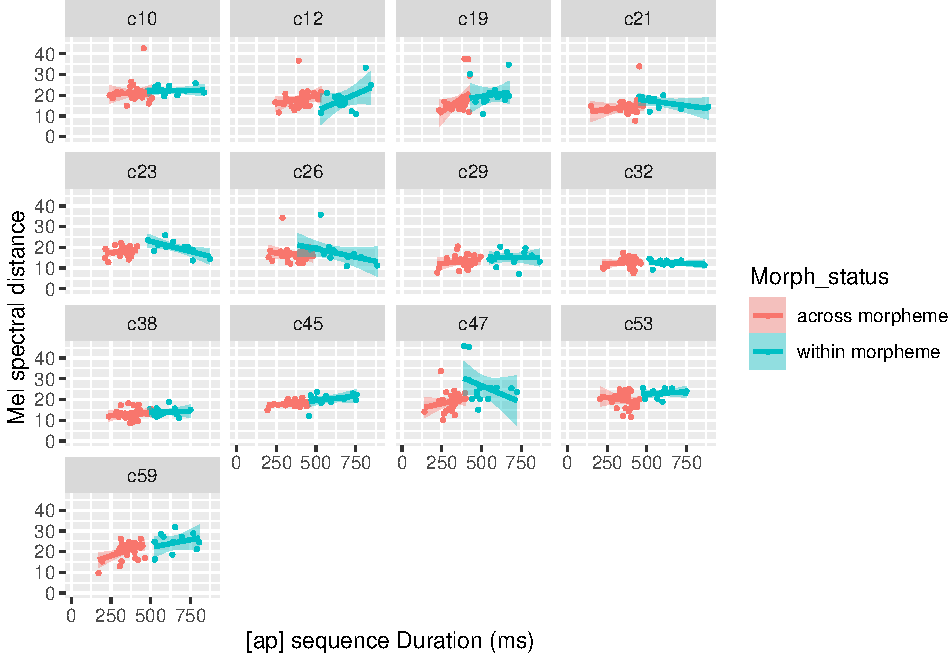
\includegraphics{3_ch3_results_files/figure-latex/seven-facet-ap-1.pdf}
\caption{\label{fig:seven-facet-ap}Coarticulation by {[}ap{]} duration, word, and morphological environment in seven-year-old children}
\end{figure}

\begin{figure}
\centering
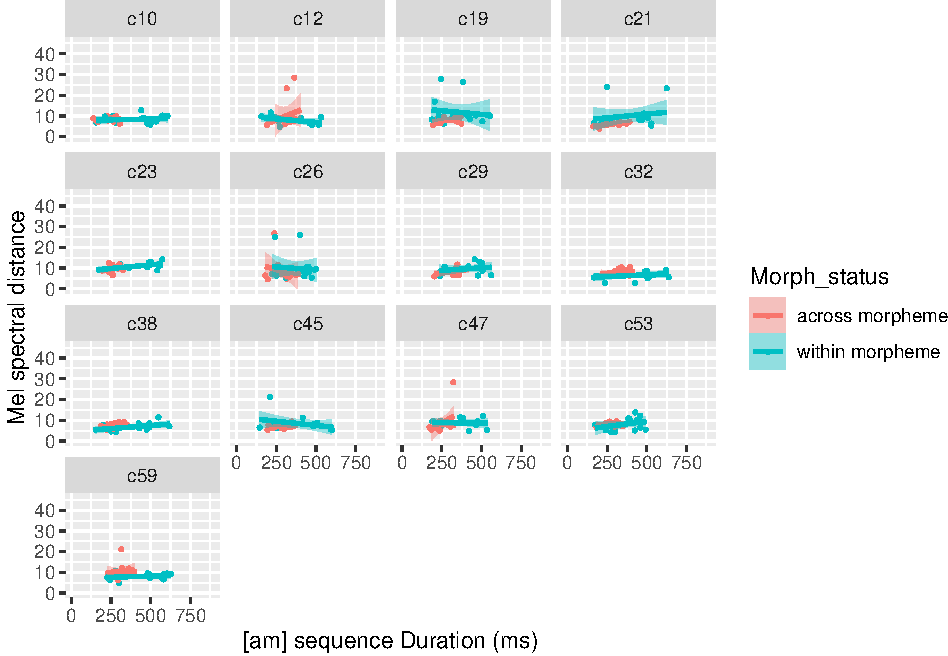
\includegraphics{3_ch3_results_files/figure-latex/seven-facet-am-1.pdf}
\caption{\label{fig:seven-facet-am}Coarticulation by {[}am{]} duration, word, and morphological environment in seven-year-old children}
\end{figure}

\begin{figure}
\centering
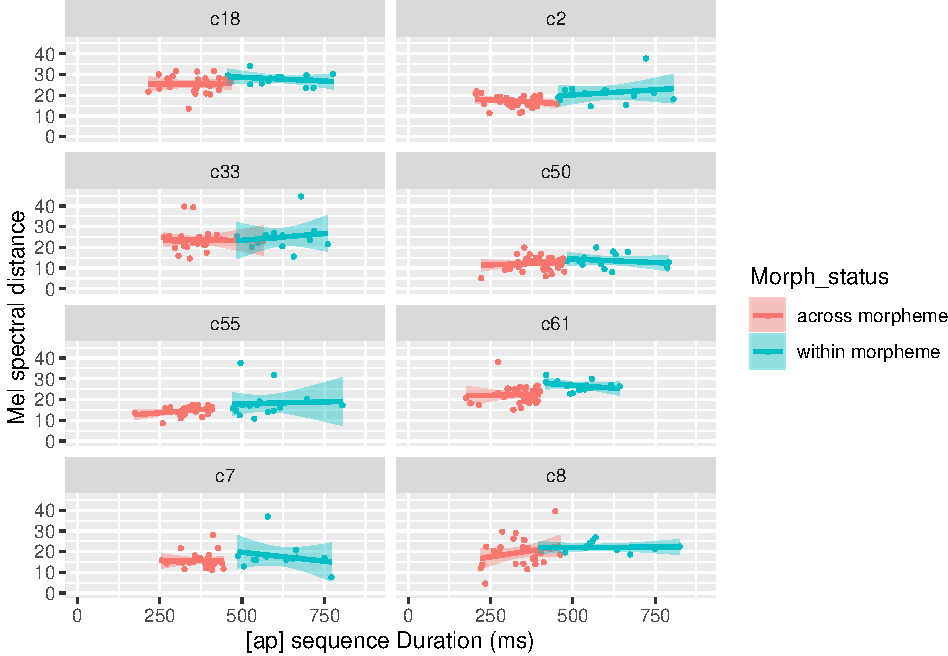
\includegraphics{3_ch3_results_files/figure-latex/eight-facet-ap-1.pdf}
\caption{\label{fig:eight-facet-ap}Coarticulation by {[}ap{]} duration, word, and morphological environment in eight-year-old children}
\end{figure}

\begin{figure}
\centering
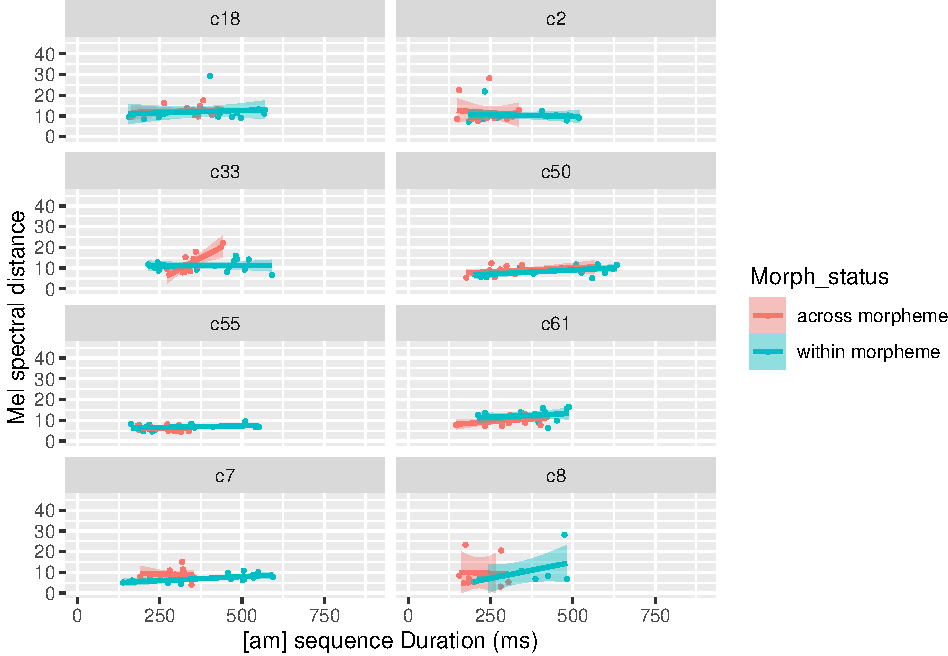
\includegraphics{3_ch3_results_files/figure-latex/eight-facet-am-1.pdf}
\caption{\label{fig:eight-facet-am}Coarticulation by {[}am{]} duration, word, and morphological environment in eight-year-old children}
\end{figure}

\begin{figure}
\centering
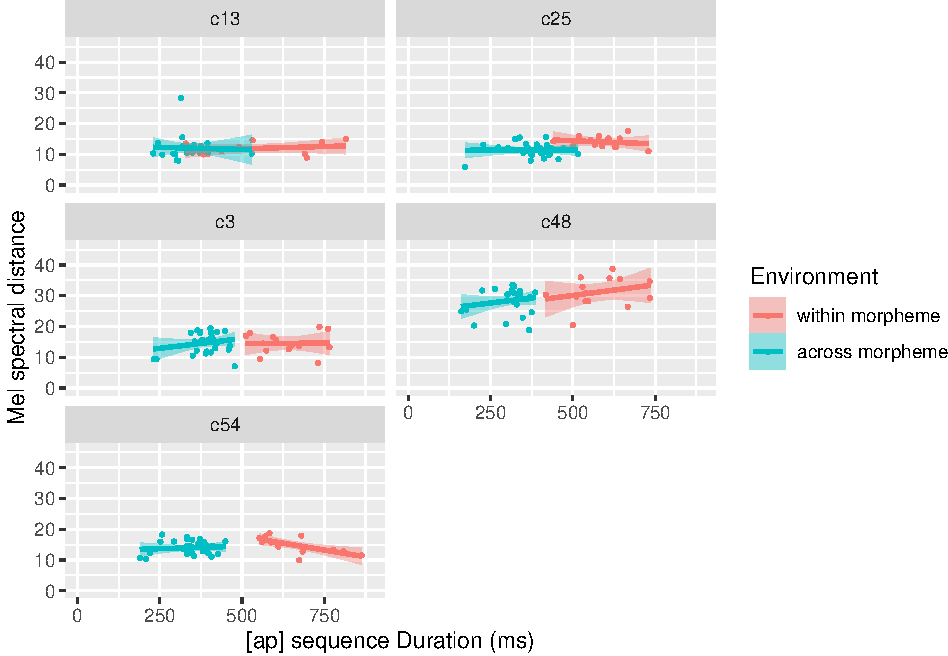
\includegraphics{3_ch3_results_files/figure-latex/nine-facet-ap-1.pdf}
\caption{\label{fig:nine-facet-ap}Coarticulation by {[}ap{]} duration, word, and morphological environment in nine-year-old children}
\end{figure}

\begin{figure}
\centering
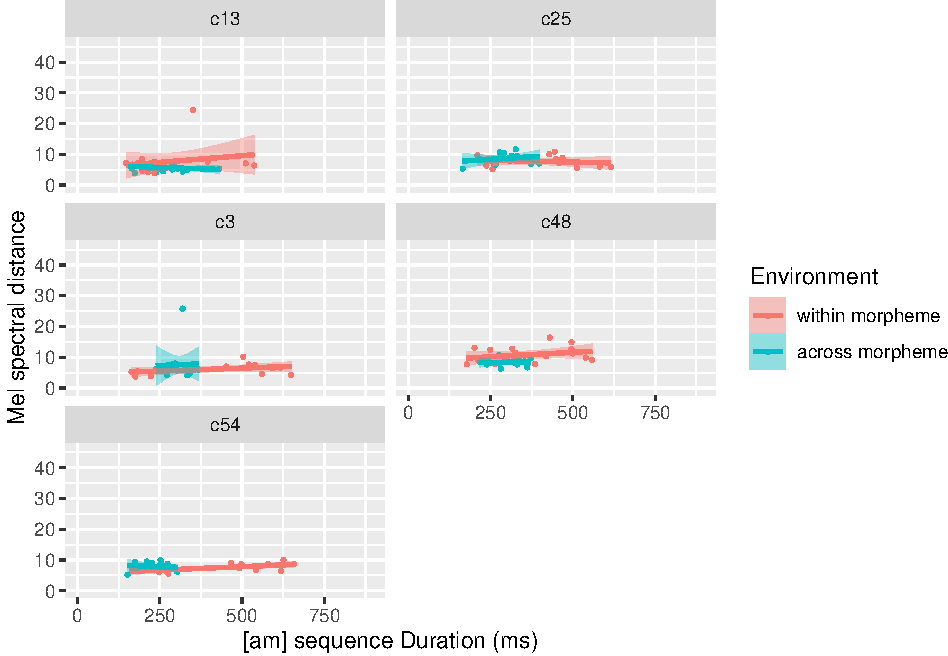
\includegraphics{3_ch3_results_files/figure-latex/nine-facet-am-1.pdf}
\caption{\label{fig:nine-facet-am}Coarticulation by {[}am{]} duration, word, and morphological environment in nine-year-old children}
\end{figure}

\begin{figure}
\centering
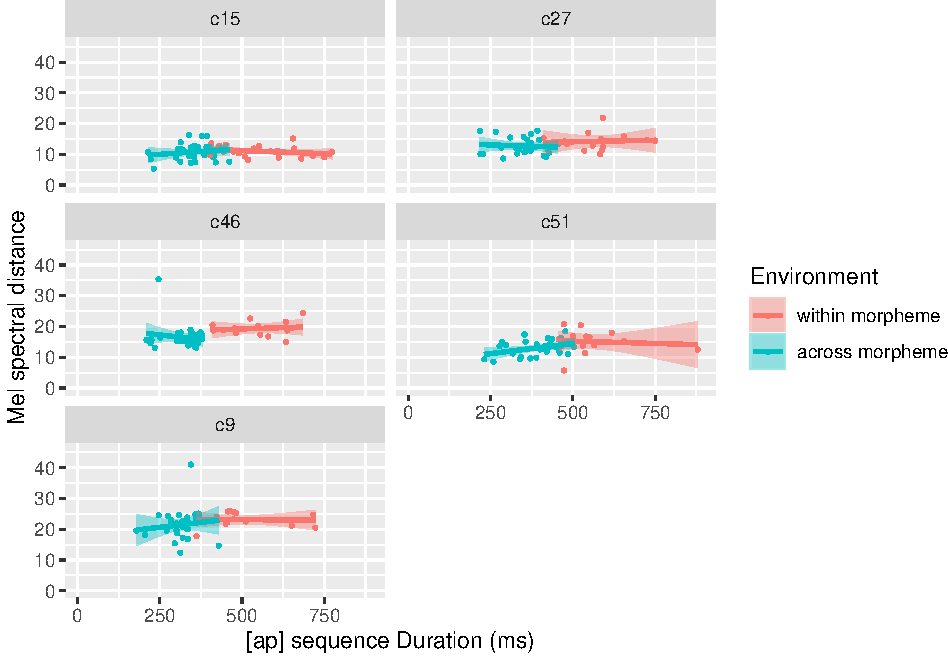
\includegraphics{3_ch3_results_files/figure-latex/ten-facet-ap-1.pdf}
\caption{\label{fig:ten-facet-ap}Coarticulation by {[}ap{]} duration, word, and morphological environment in ten-year-old children}
\end{figure}

\begin{figure}
\centering
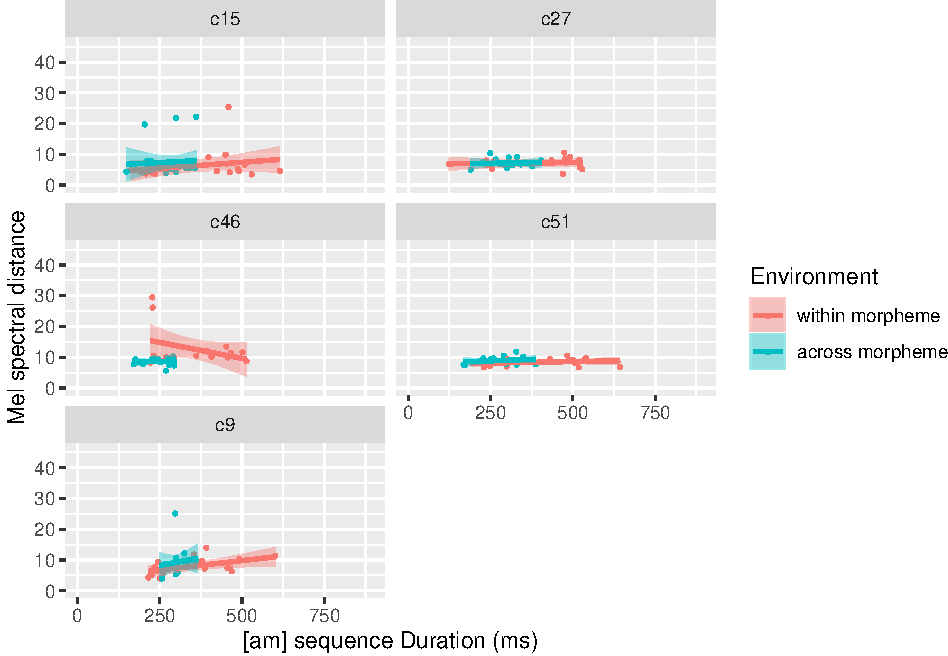
\includegraphics{3_ch3_results_files/figure-latex/ten-facet-am-1.pdf}
\caption{\label{fig:ten-facet-am}Coarticulation by {[}am{]} duration, word, and morphological environment in ten-year-old children}
\end{figure}



\end{document}


